\documentclass[11pt]{article}
\usepackage[margin=0.9in]{geometry}
\usepackage{amsmath,amssymb,graphicx,booktabs,hyperref,xcolor,float}
\usepackage[T1]{fontenc}
\hypersetup{colorlinks=true,linkcolor=blue!60!black,urlcolor=blue!60!black}
\graphicspath{{../v3/}{../cocoa/analysis/}}
\newcommand{\hmpc}{\,h\,\mathrm{Mpc}^{-1}}
\newcommand{\dchi}{\Delta\chi^2}
\title{NLA and TATT against FLAMINGO intrinsic alignments:\\ goodness of fit, $\dchi$, figure of bias and scale cuts for Roman cosmic shear}
\author{Work log, 6--7 November 2026}
\date{}
\begin{document}
\maketitle

\section*{Summary}
\begin{itemize}
\item The FLAMINGO spectra are converted to the cosmolike convention before any use (Sec.~\ref{sec:data}); the conversion is verified three ways (App.~\ref{app:checks}).
\item With the shape-noise level fixed to its B-mode value, NLA stops describing the FLAMINGO IA spectra at $k_{\max}\simeq0.09$--$0.12\hmpc$ and TATT at $0.22$--$0.29\hmpc$ at every core snapshot ($0.2\le z\le2$); combined over the core, $p<0.05$ at $k_{\max}=0.12$ (NLA) and $0.29$ (TATT). An earlier version of this test fitted a free white level per snapshot and came out two to three times more lenient, because the free level absorbed a white II excess present in FLAMINGO (Sec.~\ref{sec:white}).
\item Roman weighs the IA spectra almost entirely at $k\le0.2\hmpc$ and $z=0.75$--$2$. A unit of FLAMINGO $\chi^2$ placed at $k\simeq0.1$ is worth $\sim0.25$ of Roman $\dchi$ (summed over the 26 snapshot--spectrum cells at that $k$); at $k=0.5$ it is worth $0.01$ and at $k>1$ less than $10^{-3}$. There is no single conversion factor between $\dchi_{\rm FL}$ and $\dchi_{\rm Roman}$; the translation is a matrix (Sec.~\ref{sec:translate}).
\item In Roman $\xi_\pm$ (figure of bias, IA and $\Omega_m,A_s$ refitted) NLA and TATT are biased identically: FoB $=0.3$ at $K_0\simeq0.3$ in the production $k_{\rm UV}=K_0/D(z)$ family, or $k_{\rm UV}(z=1)\simeq0.37\hmpc$ for a cut flat in $z$. The common bias is a white (one-halo-like) E-mode II term in FLAMINGO that no single-tidal-field model has; it enters $\xi_-$ as a $\theta^{-2}$ tail that the $k$ masks do not remove. With the white term modelled (one extra linear parameter) both models are unbiased to $k_{\rm UV}(z=1)\simeq0.3$--$0.4\hmpc$ and TATT is the better model beyond that, as expected.
\item The Roman test proper (all parameters free with the chain priors, controls at every mask, Sec.~\ref{sec:romantest}): cases A and B agree; FoB $=0.3$ at $K_0\simeq0.3$ or a flat $k_{\rm UV}\simeq0.37\hmpc$ for both models; the matched-model and injection controls are zero. An MCMC at $K_0=0.3$ reproduces the MAP shifts and shows a $0.24\sigma$ prior-volume shift for TATT even on a TATT truth, so MAP (or control-subtracted) shifts are the right statistic.
\item The purely simulation-based cuts are $k_{\max}(z)\simeq0.1\hmpc$ (NLA) and $0.25$--$0.3\hmpc$ (TATT), both nearly flat in $z$ over $0.2\le z\le2$: they do not follow the $K_0/D(z)$ scaling of the production masks, which changes by a factor 2.2 over the same range (Sec.~\ref{sec:kuvz}). In Roman the NLA cut leaves 9 of 1080 $\xi_\pm$ points; the TATT cut leaves 145 and gives FoB $0.22\pm0.09$ for either model.
\end{itemize}

\section{Data and conversion}\label{sec:data}
FLAMINGO L1000N1800 (box $681\,h^{-1}$Mpc), 13 snapshots $z=0$--$4$, folds 1/4/16 combined ($k<1.2$, $1.2$--$9$, $>9\hmpc$), measured $P_{hh}$, $P_{hE}^{(0)}$, $P_{EE}^{(0,2,4)}$, $P_{BB}^{(0,2,4)}$ with mode-scatter error bars. Conversion to the cosmolike ($\mu=0$, shear) convention, with $R=1-e_{\rm rms}^2$ and $\langle W^2_{\rm NGP}\rangle$ the NGP window:
\begin{align}
P_{\delta E}(k) &= \frac{3}{2}\,\frac{M_0^{hE}(k)}{2R}\,\frac{1}{b(k)},\qquad b(k)=\sqrt{\frac{P_{hh}(k)-1/\bar n}{P_{\rm NL}(k)}},\\
P_{EE}(k) &= \frac{M_0^{EE}-\tfrac52 M_2^{EE}+\tfrac{27}{8}M_4^{EE}}{(2R)^2\,\langle W^2_{\rm NGP}\rangle},\qquad P_{BB}\ \text{likewise},\\
N_s &= \mathrm{median}_{5<k<10}\,P_{BB}^{\rm nfold\,4}(k)\quad\text{(white shape-noise level, E = B for isotropic shapes).}
\end{align}
$\bar n=N_{\rm gal}/L^3$ and $e_{\rm rms}$ are taken from the \texttt{hinfo} files of the same runs (\texttt{Galaxy\_DS\_Field}): $N_{\rm gal}$ agrees exactly with the table used (no galaxies dropped, \texttt{ngal\_used} $=$ \texttt{ngal}), and the per-component rms ellipticity agrees to its three decimals on all three projection axes (e.g.\ $z=1$: $e_{1z},e_{2z}=0.3048,0.3051$ against 0.305); the six-decimal values change $R$ by $0.01\%$. The 858 spectrum files supplied on 7 November are byte-identical to those used. The low-$k$ NLA amplitude recovered from these spectra reproduces the 27 October report to 0.1--1.1\% at all 13 snapshots; the same conversion applied inside \texttt{sim\_IA.c} gives the same Roman $\xi_{\rm IA}$ to $2.5\times10^{-9}$ (App.~\ref{app:checks}).

\paragraph{Snapshot selection.} Table~\ref{tab:snaps}. The core set is $0.2\le z\le2$: $z=0,0.1$ have 2--4~M galaxies and carry $<0.1\%$ of Roman's weight (Sec.~\ref{sec:translate}); $z=3,4$ have 0.5--1.6~M galaxies, $1/\bar n$ of 200--600 $(h^{-1}{\rm Mpc})^3$, and $<1\%$ of the weight. The null spectra $P_{hB}$, $P_{EB}$ are consistent with zero at every snapshot (rms$/\sigma$ 0.4--1.7 over $k<0.3$). At $z=2$ the bounded TATT fit flips to $a_2>0$, $b_{\rm TA}=0$; it is kept in the cuts but excluded from the $A_2(z)$ power law.

\begin{table}[H]\centering\small
\begin{tabular}{rrrrrrrr}
\toprule
$z$ & $N_{\rm gal}$ [M] & $e_{\rm rms}$ & $1/\bar n$ & $N_s$ & $X/N_s$ & $N_s^{\rm free}/N_s$ & core\\
\midrule
0.0 & 2.03 & 0.250 & 155 & 0.020 & 4.9 & 4.8 & \\
0.1 & 3.69 & 0.254 & 86 & 0.027 & 2.6 & 3.4 & \\
0.2 & 5.53 & 0.262 & 57 & 0.043 & 3.2 & 2.9 & $\checkmark$\\
0.3 & 5.77 & 0.268 & 55 & 0.050 & 2.5 & 2.9 & $\checkmark$\\
0.4 & 5.85 & 0.274 & 54 & 0.055 & 1.8 & 2.8 & $\checkmark$\\
0.5 & 5.93 & 0.280 & 53 & 0.063 & 2.5 & 2.7 & $\checkmark$\\
0.6 & 5.93 & 0.285 & 53 & 0.066 & 2.3 & 2.8 & $\checkmark$\\
0.75 & 5.88 & 0.293 & 54 & 0.075 & 1.5 & 2.3 & $\checkmark$\\
1.0 & 5.66 & 0.305 & 56 & 0.088 & 1.7 & 2.4 & $\checkmark$\\
1.5 & 4.81 & 0.323 & 66 & 0.127 & 1.9 & 2.1 & $\checkmark$\\
2.0 & 3.66 & 0.335 & 86 & 0.186 & 1.9 & 2.3 & $\checkmark$\\
3.0 & 1.61 & 0.358 & 196 & 0.410 & 2.2 & 2.8 & \\
4.0 & 0.53 & 0.371 & 592 & 0.747 & 2.9 & 3.7 & \\
\bottomrule
\end{tabular}
\caption{Snapshots. $1/\bar n$ and $N_s$ in $(h^{-1}{\rm Mpc})^3$. $X$ is the white II excess of Sec.~\ref{sec:white}; $N_s^{\rm free}$ the white level a free nuisance fits (v2, NLA, $k_{\max}=0.22$).}
\label{tab:snaps}
\end{table}

\section{Models and fits}
NLA and TATT at the FLAMINGO cosmology (CAMB, halofit Takahashi, FAST-PT kernels), per snapshot, with $x\equiv(1+z)/1.62$:
\begin{align}
C_1 &= a_1\,\frac{\Omega_m\,\bar C_1\rho_{\rm crit}}{D(z)},\qquad C_2 = a_2\,\frac{\Omega_m\,\bar C_1\rho_{\rm crit}}{D(z)^2},\qquad \bar C_1\rho_{\rm crit}=0.01389,\\
\text{NLA:}\quad P_{\delta E}&=-C_1P_{\rm NL},\qquad P_{EE}=C_1^2P_{\rm NL},\qquad P_{BB}=0,\\
\text{TATT:}\quad P_{\delta E}&=-C_1P_{\rm NL}+C_1 b_{\rm TA}\,A_{0|0E}+C_2\,(\ldots),\quad P_{EE},\ P_{BB}\ \text{with the } A_{0|0E},\,A_{E2}\ldots\ \text{FAST-PT kernels.}
\end{align}
The observed-unit model is $\{b(k)P_{\delta E},\ P_{EE}+N_s,\ P_{BB}+N_s\}$. Per snapshot and $k_{\max}$ the parameters $\{a_1\}$ (NLA) or $\{a_1,a_2,b_{\rm TA}\}$ (TATT) are fitted over $0.05\le k\le k_{\max}$ by least squares with the measured errors, bounded to the chain priors ($|a_2|\le5$, $0\le b_{\rm TA}\le2$), from several starts. \textbf{$N_s$ is held at its B-mode value.} In the Roman fits the models are cosmolike's own NLA/TATT with $A_i(z)=A_i\,x^{\eta_i}$, so $(A_1,\eta_1)$ and $(A_2,\eta_2,b_{\rm TA})$ are fitted jointly together with $\Omega_m$ and $A_s$.

\section{Goodness of fit versus $k_{\max}$ in FLAMINGO}\label{sec:gof}
Per snapshot, $\chi^2(k_{\max})$ of the refit against the measured spectra, dof $=3N_k-N_{\rm par}$, $p=P(\chi^2_{\rm dof}>\chi^2)$; the cut is the last $k_{\max}$ before two consecutive $p<0.05$. Three further criteria, all from the simulation alone:
\begin{enumerate}
\item \textbf{Anchored}: parameters fixed by the fit to $k\le0.16\hmpc$ (large scales), cumulative $p$ of the extrapolation to $k_{\max}$. A model that is right on large scales but drifts is caught here; the refit can hide drift by compromising the amplitude.
\item \textbf{Fractional accuracy}: anchored model against the noise-free (smoothed) spectra, $\max_{k\le k_{\max}}|M/T-1|\le 5\%$ (or 10\%), for GI ($bP_{\delta E}$) and II ($P_{EE}-N_s$) separately. Insensitive to the simulation error bars (which are tiny at high $k$), it asks how accurate the model is, not how significant the misfit.
\item $\dchi_{\rm FL}(k_{\max})$: refit against the noise-free spectra, FLAMINGO errors, summed over the core (Fig.~\ref{fig:dfl}); the quantity that can be translated to Roman.
\end{enumerate}

\begin{figure}[H]\centering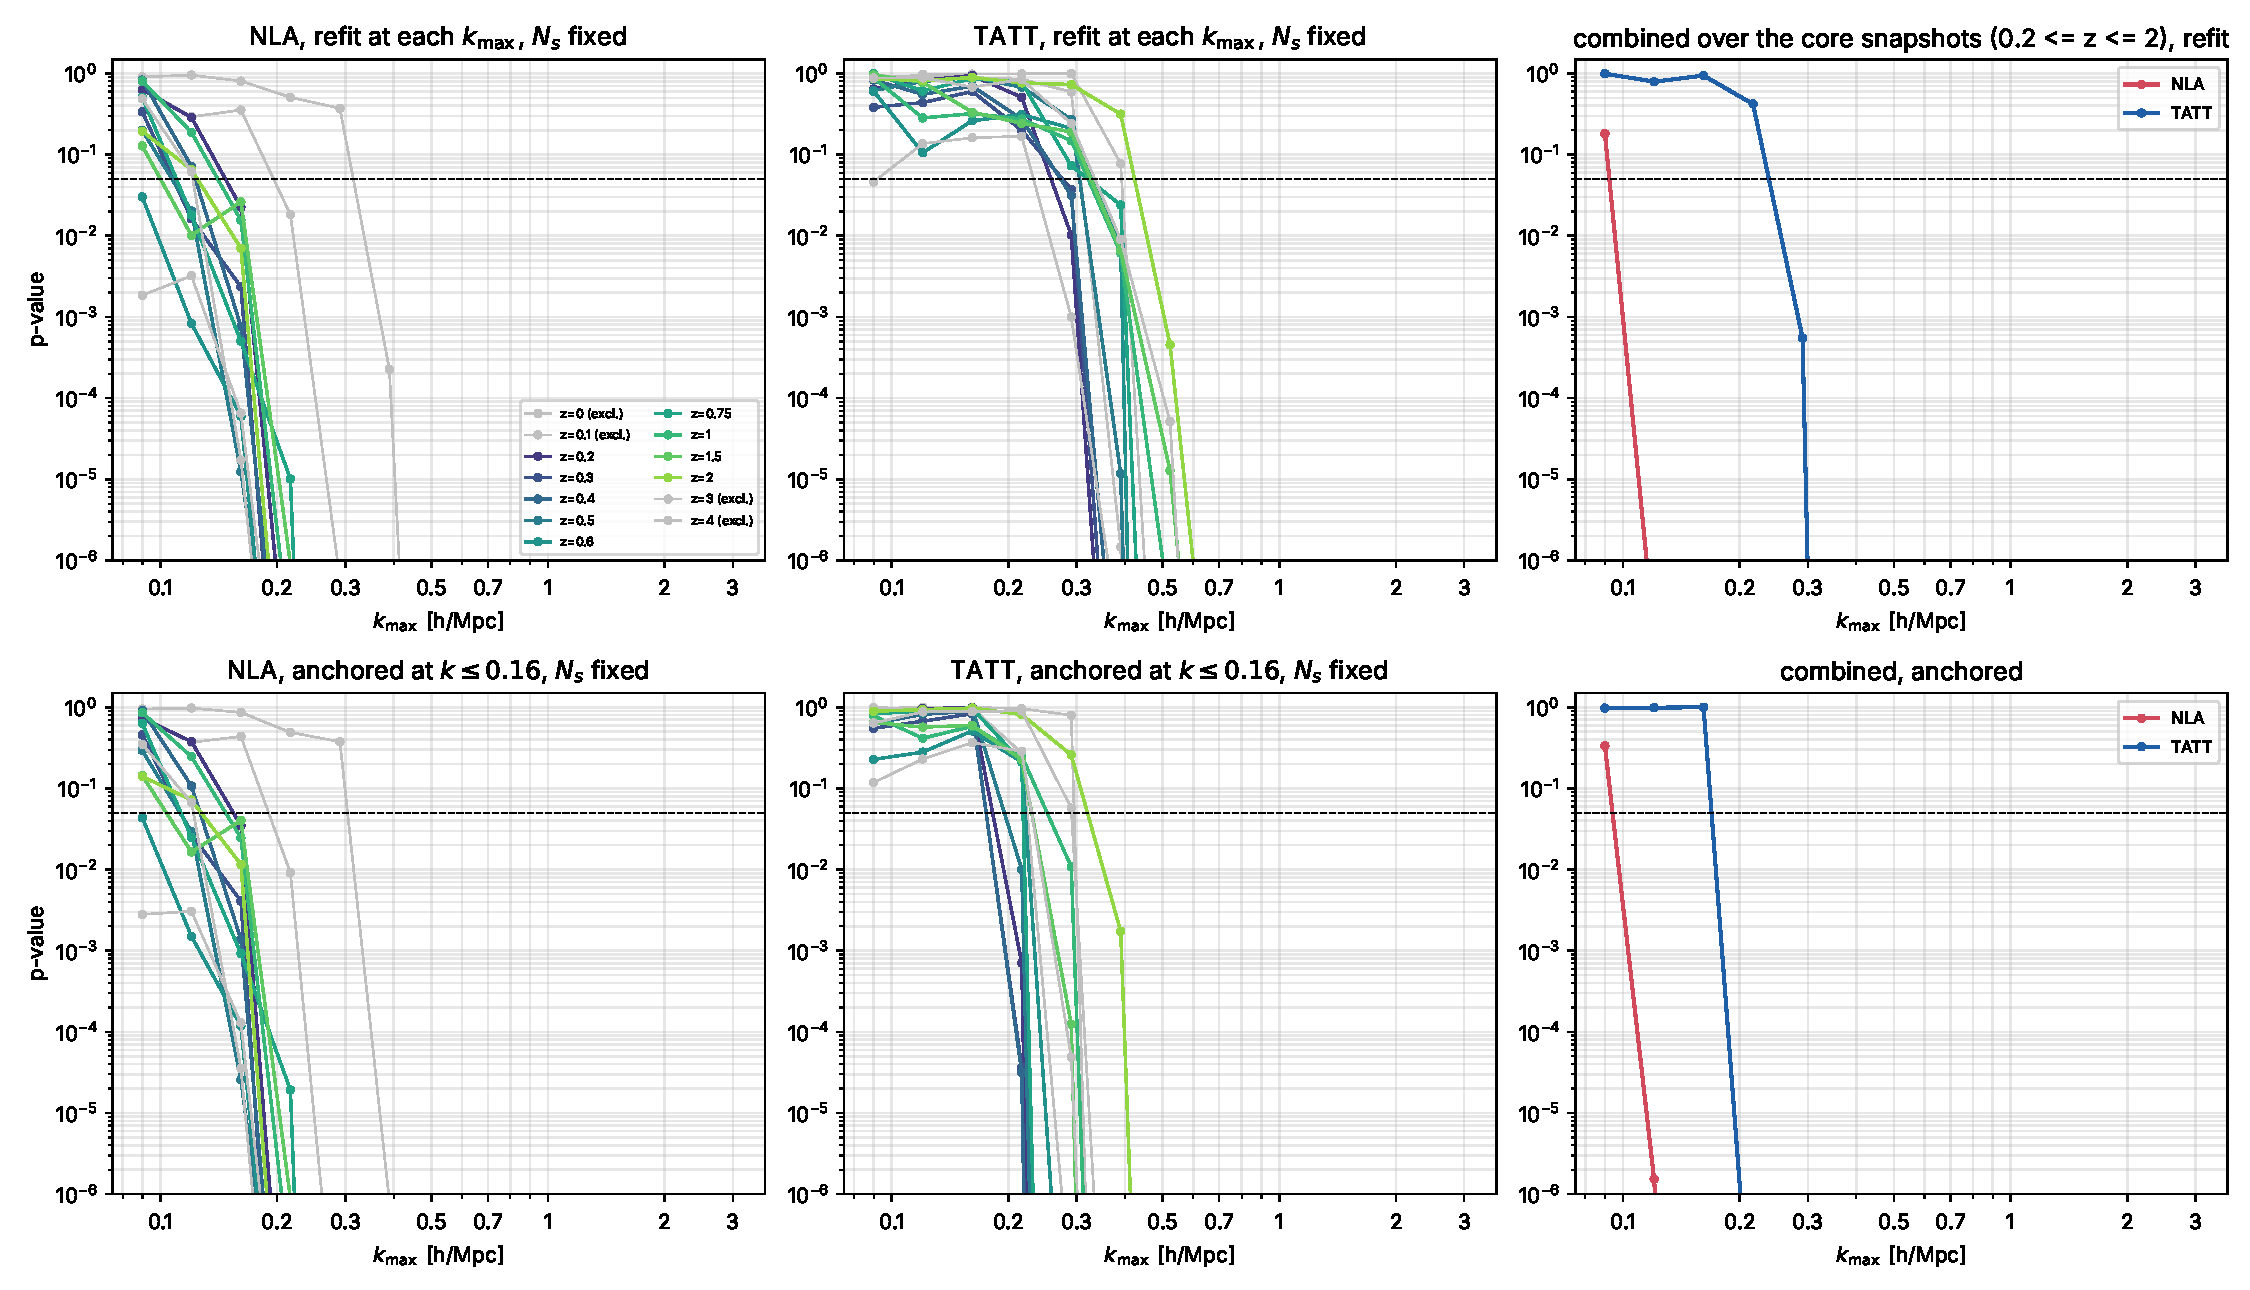
\includegraphics[width=\textwidth]{fig_v3_gof.pdf}
\caption{$p$-values versus $k_{\max}$, $N_s$ fixed. Top: refit at each $k_{\max}$; bottom: anchored at $k\le0.16$. Grey: excluded snapshots. Right: combined over the core.}\label{fig:gof}\end{figure}

\begin{figure}[H]\centering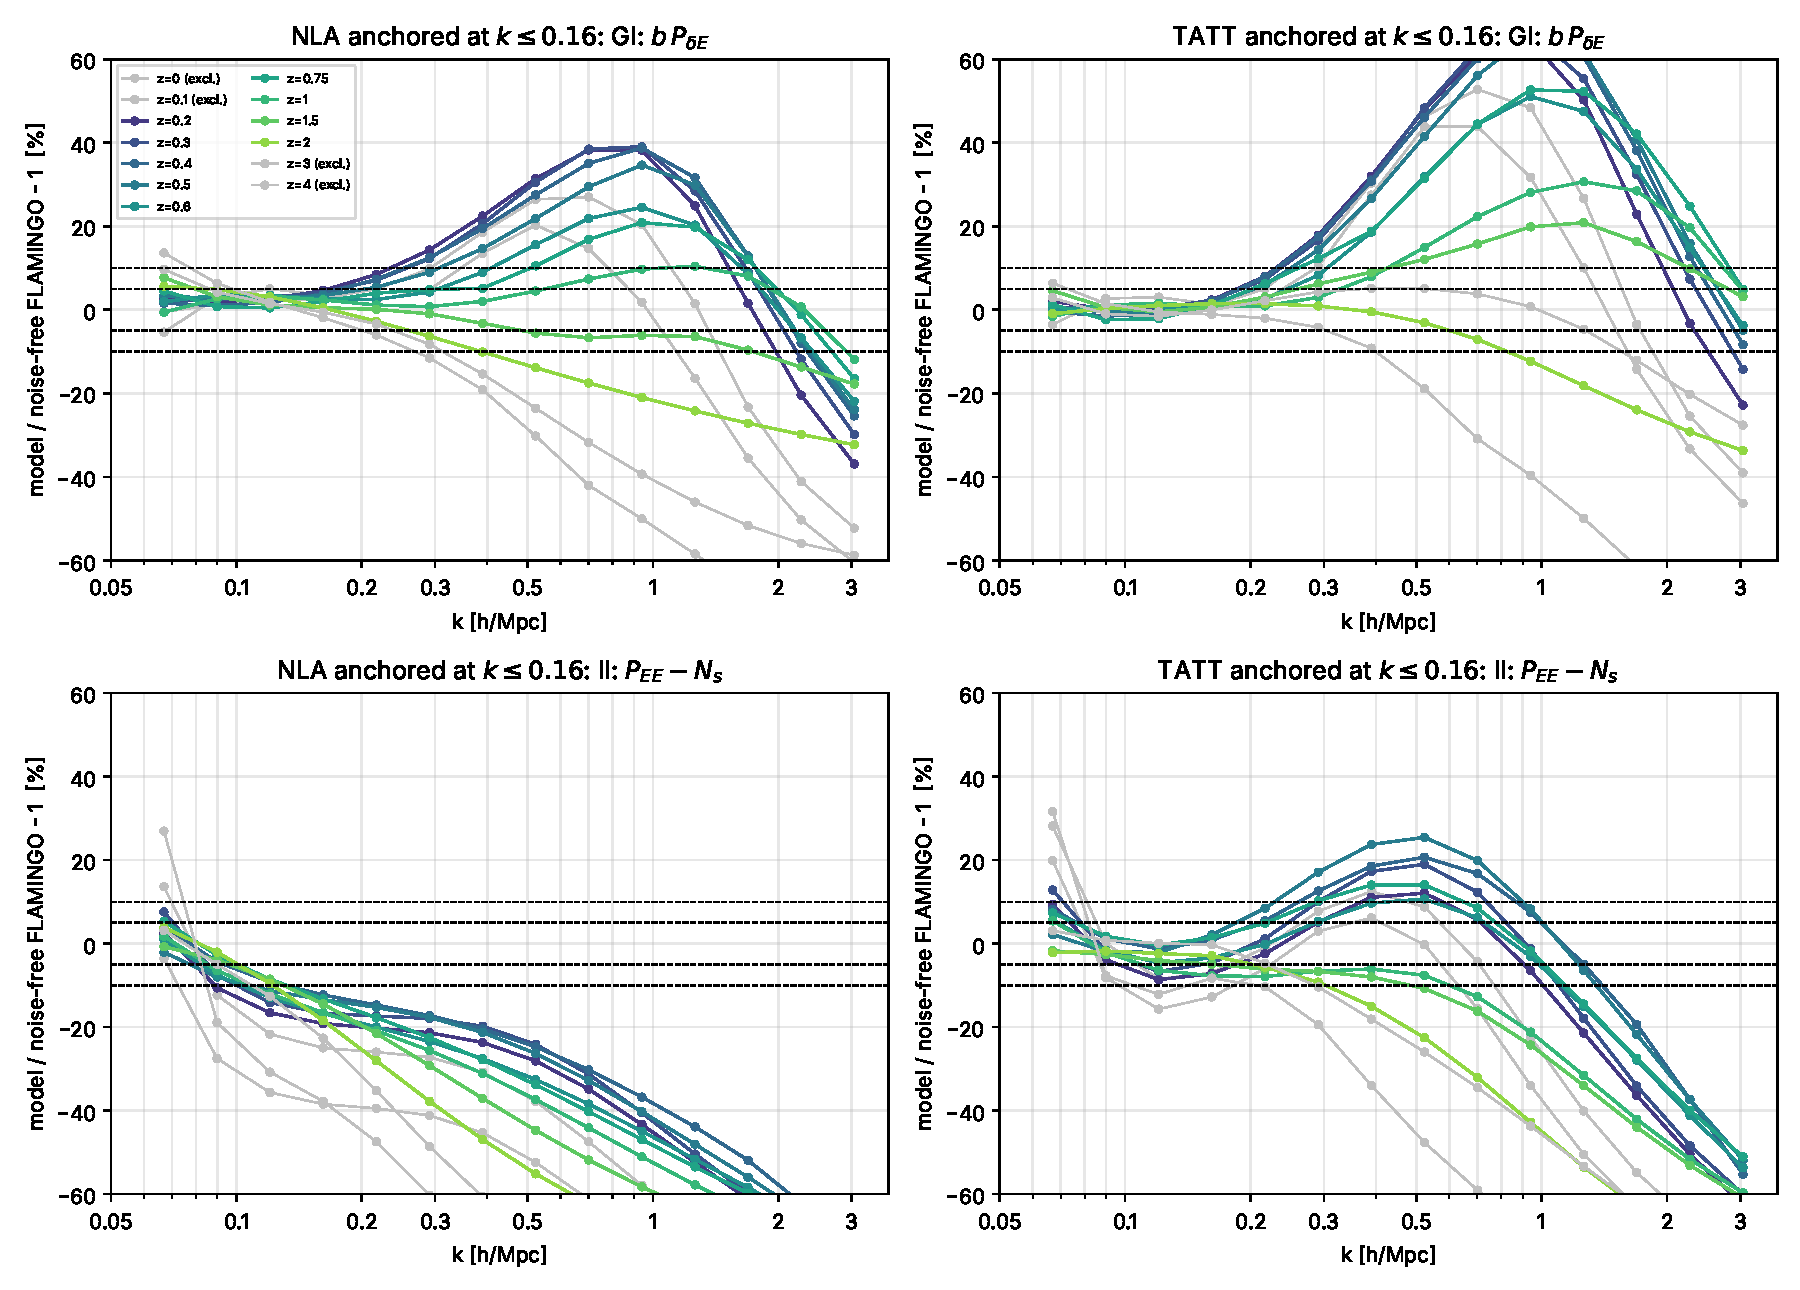
\includegraphics[width=\textwidth]{fig_v3_deviation.pdf}
\caption{Anchored model over the noise-free FLAMINGO spectra. NLA's GI holds to 5\% up to $k\simeq0.2$; its II is 10\% low already at $k=0.12$ (the white excess). TATT's GI holds to $\simeq0.25$, its II to 10\% up to $\simeq0.3$.}\label{fig:dev}\end{figure}

\begin{table}[H]\centering\small
\begin{tabular}{r|cccc|cccc}
\toprule
 & \multicolumn{4}{c|}{NLA $k_{\max}$ [$h$/Mpc]} & \multicolumn{4}{c}{TATT $k_{\max}$ [$h$/Mpc]}\\
$z$ & GoF & anchored & 5\% GI & 10\% & GoF & anchored & 5\% GI & 10\%\\
\midrule
0.2 & 0.12 & 0.12 & 0.16 & -- & 0.22 & 0.16 & 0.16 & 0.22\\
0.3 & 0.09 & 0.09 & 0.16 & 0.09 & 0.22 & 0.16 & 0.16 & --\\
0.4 & 0.12 & 0.12 & 0.16 & 0.12 & 0.22 & 0.16 & 0.16 & 0.22\\
0.5 & 0.09 & 0.09 & 0.16 & 0.09 & 0.29 & 0.16 & 0.16 & 0.22\\
0.6 & $<$0.09 & $<$0.09 & 0.29 & 0.09 & 0.29 & 0.22 & 0.22 & 0.29\\
0.75 & 0.09 & 0.09 & 0.29 & 0.12 & 0.29 & 0.22 & 0.16 & 0.22\\
1.0 & 0.12 & 0.12 & 0.52 & 0.09 & 0.29 & 0.22 & 0.29 & 0.39\\
1.5 & 0.09 & 0.09 & -- & 0.12 & 0.29 & 0.22 & 0.22 & 0.39\\
2.0 & 0.12 & 0.12 & -- & 0.12 & 0.39 & 0.29 & 0.52 & 0.29\\
\midrule
combined & 0.09 & 0.09 & & & 0.22 & 0.16 & & \\
\bottomrule
\end{tabular}
\caption{Per-snapshot cuts (core). ``--'': the criterion is not met at the smallest $k_{\max}$ (0.09). The 5\% II criterion is met nowhere for either model because of the white excess. ``combined'': last $k_{\max}$ with the core-summed $p\ge0.05$ (NLA: $p=0.18$ at 0.09, $10^{-7}$ at 0.12; TATT: 0.42 at 0.22, $5\times10^{-4}$ at 0.29).}
\label{tab:cuts}
\end{table}

\begin{figure}[H]\centering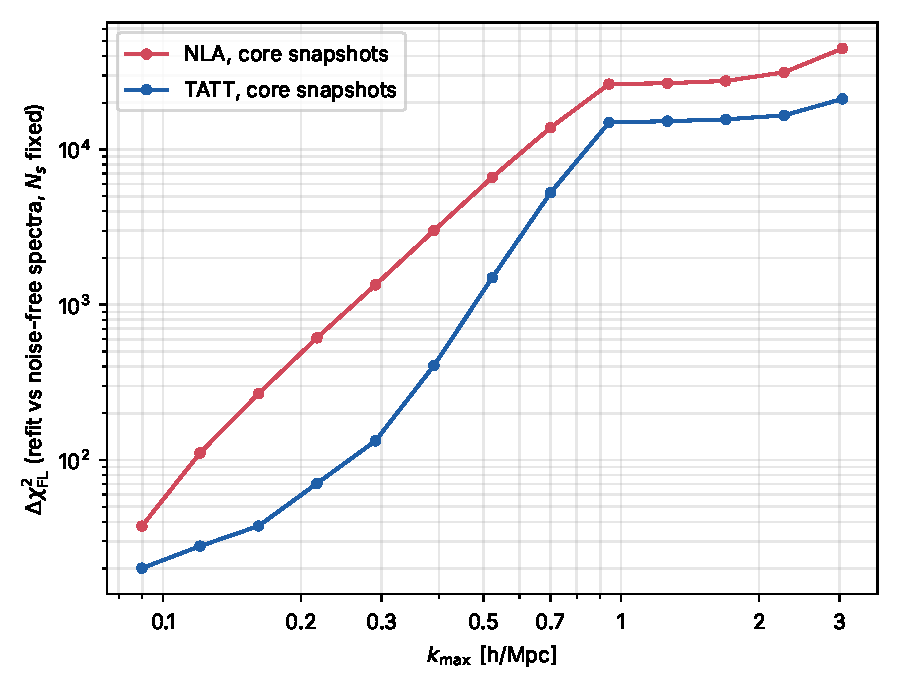
\includegraphics[width=0.48\textwidth]{fig_v3_dchi2fl.pdf}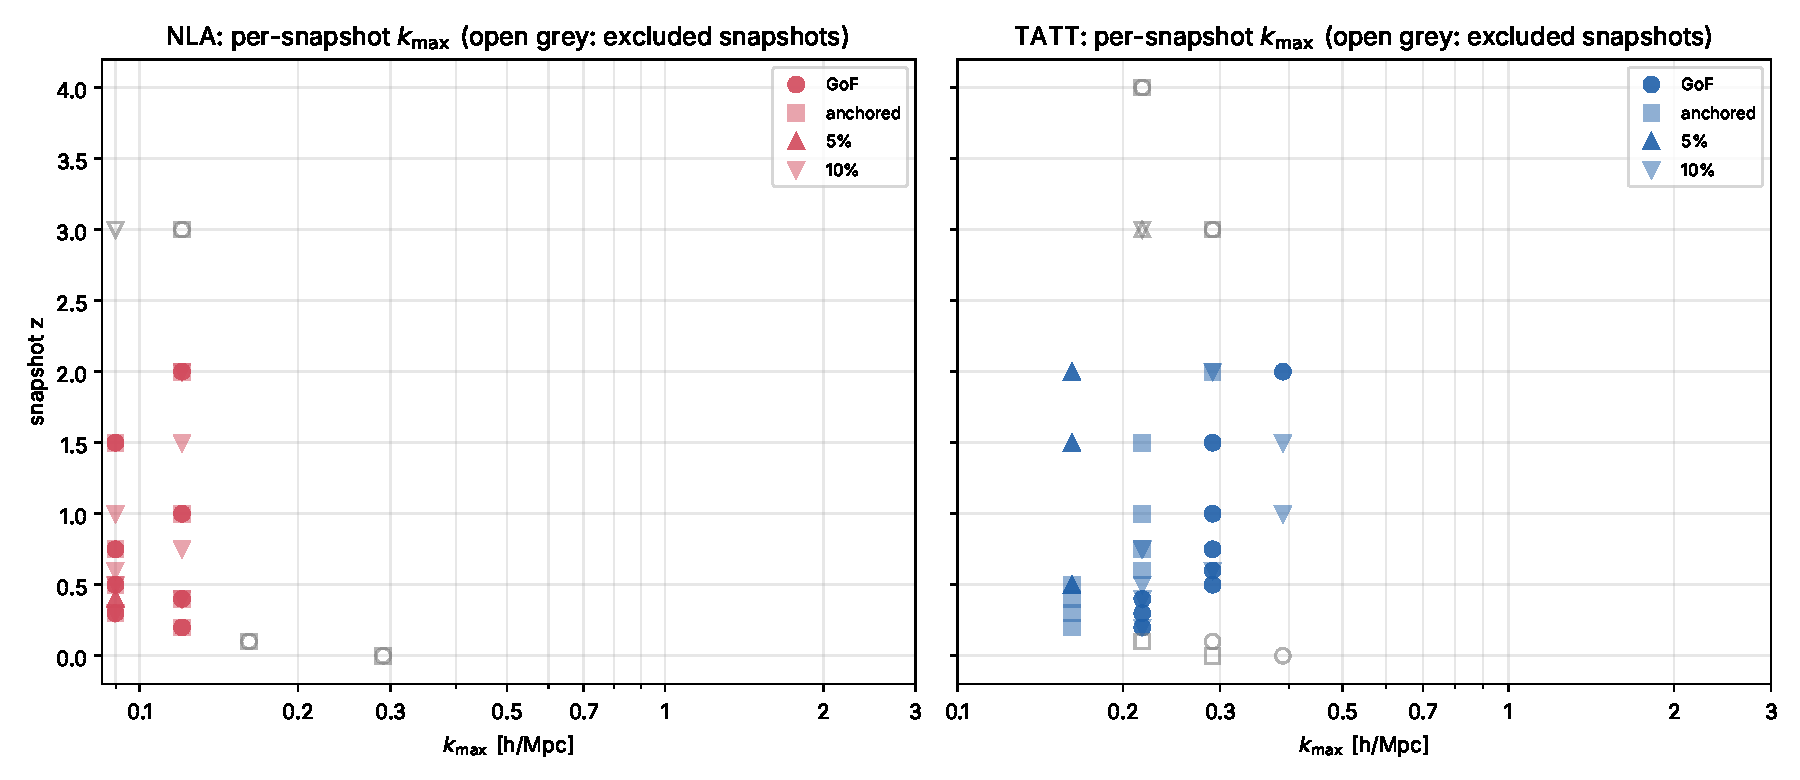
\includegraphics[width=0.5\textwidth]{fig_v3_cuts.pdf}
\caption{Left: $\dchi_{\rm FL}(k_{\max})$, core sum, $N_s$ fixed. Right: per-snapshot cuts by criterion ($k_{\max}$ horizontal, $z$ vertical).}\label{fig:dfl}\end{figure}

\section{Amplitude evolution $A_1(z)$, $A_2(z)$}
Fig.~\ref{fig:amp}, Table~\ref{tab:amp}. From the anchored fits ($k\le0.16$), power laws over $0.2\le z\le1.5$:
\begin{align}
\text{NLA:}\quad A_1(z)&=(3.66\pm0.01)\,x^{\,0.56\pm0.02},\\
\text{TATT:}\quad A_1(z)&=(3.66\pm0.04)\,x^{\,0.50\pm0.05},\qquad A_2(z)=(-0.93\pm0.06)\,x^{\,0.01\pm0.31},\qquad b_{\rm TA}\simeq0.37\pm0.03\ \text{(mean)}.
\end{align}
Including $z=2$ steepens NLA to $3.68\,x^{0.62}$ and breaks the $A_2$ law ($z=2$ gives $a_2=+2.0$ at the $b_{\rm TA}=0$ bound). The Roman fit of the FLAMINGO data vector ($3.5\,x^{0.68}$) agrees with the simulation's own $A_1(z)$ to 5\%; TATT's Roman fit returns $A_2\simeq0$ because the Roman data are not sensitive to $A_2$ at the scales kept (Sec.~\ref{sec:roman}).

\begin{figure}[H]\centering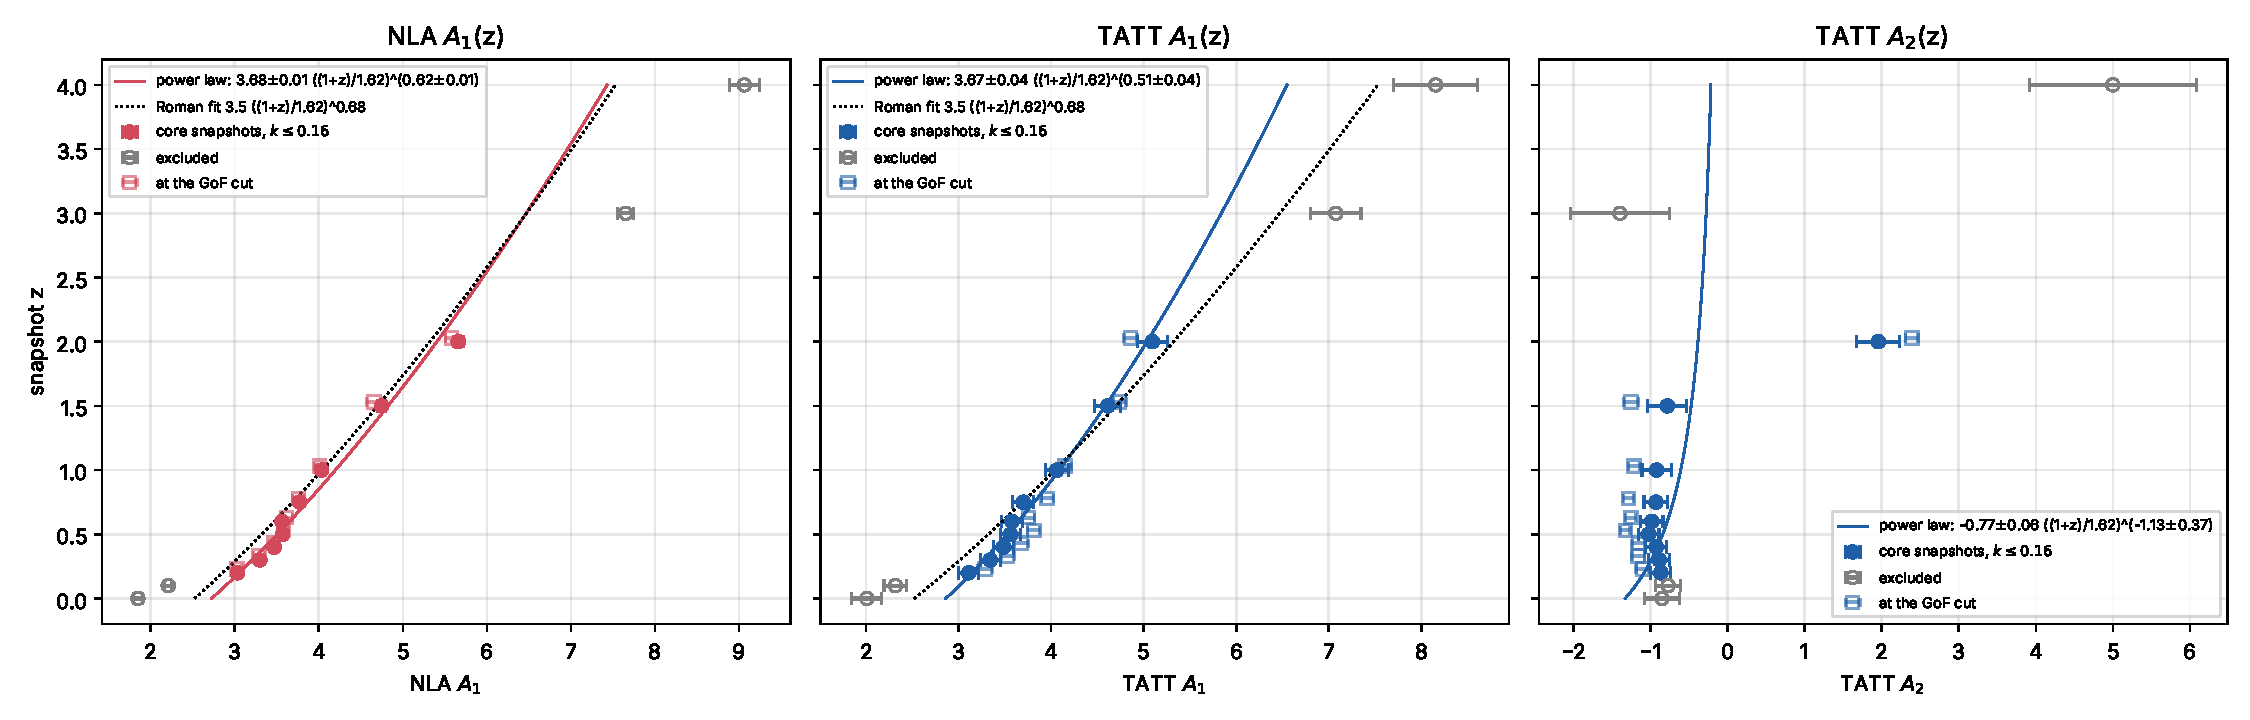
\includegraphics[width=\textwidth]{fig_v3_amplitudes.pdf}
\caption{$A_1(z)$ and $A_2(z)$ (amplitude horizontal, $z$ vertical). Filled: anchored fits; open squares: at the snapshot's GoF cut; grey: excluded snapshots.}\label{fig:amp}\end{figure}
\begin{figure}[H]\centering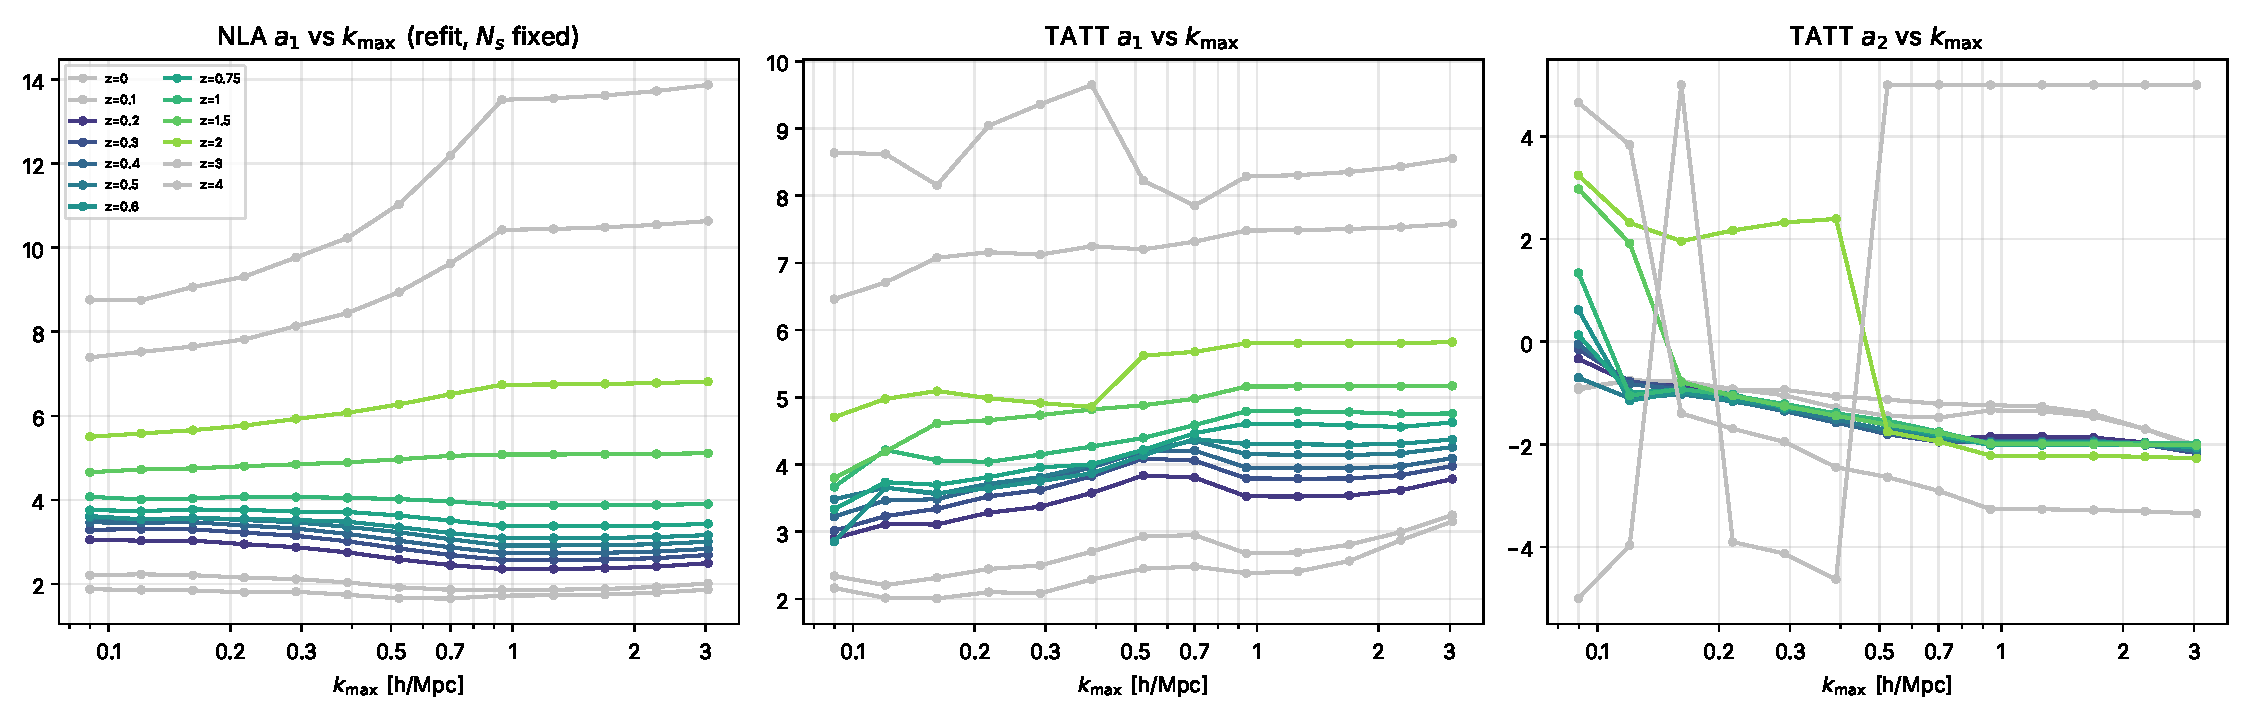
\includegraphics[width=\textwidth]{fig_v3_amp_vs_kmax.pdf}
\caption{Refit amplitudes versus $k_{\max}$, one line per snapshot.}\end{figure}

\begin{table}[H]\centering\small
\begin{tabular}{r|cc|cccc}
\toprule
$z$ & NLA $a_1$ (anchor) & NLA $a_1$ (at cut) & TATT $a_1$ & $a_2$ & $b_{\rm TA}$ & TATT cut\\
\midrule
0.2 & $3.03\pm0.04$ & $3.03\pm0.05$ & $3.11\pm0.11$ & $-0.87\pm0.13$ & $0.26\pm0.07$ & 0.22\\
0.3 & $3.30\pm0.04$ & $3.29\pm0.07$ & $3.34\pm0.11$ & $-0.89\pm0.13$ & $0.29\pm0.07$ & 0.22\\
0.4 & $3.47\pm0.04$ & $3.46\pm0.05$ & $3.49\pm0.11$ & $-0.93\pm0.13$ & $0.32\pm0.07$ & 0.22\\
0.5 & $3.57\pm0.04$ & $3.58\pm0.07$ & $3.56\pm0.11$ & $-1.02\pm0.13$ & $0.38\pm0.08$ & 0.29\\
0.6 & $3.56\pm0.04$ & $3.62\pm0.07$ & $3.58\pm0.11$ & $-0.98\pm0.15$ & $0.36\pm0.09$ & 0.29\\
0.75 & $3.77\pm0.04$ & $3.76\pm0.07$ & $3.70\pm0.11$ & $-0.93\pm0.16$ & $0.46\pm0.10$ & 0.29\\
1.0 & $4.03\pm0.04$ & $4.01\pm0.05$ & $4.06\pm0.12$ & $-0.92\pm0.19$ & $0.34\pm0.12$ & 0.29\\
1.5 & $4.75\pm0.05$ & $4.66\pm0.09$ & $4.61\pm0.14$ & $-0.78\pm0.25$ & $0.58\pm0.18$ & 0.29\\
2.0 & $5.66\pm0.06$ & $5.58\pm0.08$ & $5.09\pm0.16$ & $+1.96\pm0.28$ & $0.00\pm0.24$ & 0.39\\
\bottomrule
\end{tabular}
\caption{Amplitudes (core snapshots). TATT columns: anchored fit ($k\le0.16$); TATT cut: GoF $k_{\max}$ in $h$/Mpc.}\label{tab:amp}
\end{table}

\section{The white II excess}\label{sec:white}
Any model in which GI and II come from one tidal field obeys $P_{EE}P_{\rm NL}/P_{\delta E}^2=1$ at leading order. FLAMINGO does not:
\begin{equation}
X(k)\equiv(P_{EE}-N_s)-\frac{P_{\delta E}^2}{P_{\rm NL}}\simeq{\rm const}\ \text{in }k,\qquad X\simeq(1\text{--}2)\,N_s\quad(z\le2),
\end{equation}
flat within errors from $k=0.07$ to $0.5\hmpc$ at every snapshot (Fig.~\ref{fig:white}, left). The E-mode white power exceeds the B-mode white power by a factor 2--4: small-scale (one-halo-like) alignments, not shape noise. A free $N_s$ absorbs it (Table~\ref{tab:snaps}, last column), which is what made the earlier GoF lenient. Its Roman signature is fixed by the Limber integral: a white $P_{EE}$ gives a constant $C_\ell=X\!\int\! d\chi\,n_i n_j/\chi^2$, and
\begin{equation}
\xi_+(\theta)=\int\!\frac{\ell\,d\ell}{2\pi}J_0(\ell\theta)\,C=0\ (\theta>0),\qquad
\xi_-(\theta)=\int\!\frac{\ell\,d\ell}{2\pi}J_4(\ell\theta)\,C=\frac{2C}{\pi\theta^2},
\end{equation}
which cosmolike reproduces exactly (Fig.~\ref{fig:white}, middle): in the (0,0) bin the term is $2\sigma$ at $63'$ and $1\sigma$ at $116'$, so a $k$-based mask removes only part of it. The injected truth decomposes as (FoB, NLA/TATT, mask $0.35/D$): single tidal field 0.10/0.09; plus the excess as exactly white 0.30/0.34; plus its measured $k$ structure (production) 0.39/0.42.

\begin{figure}[H]\centering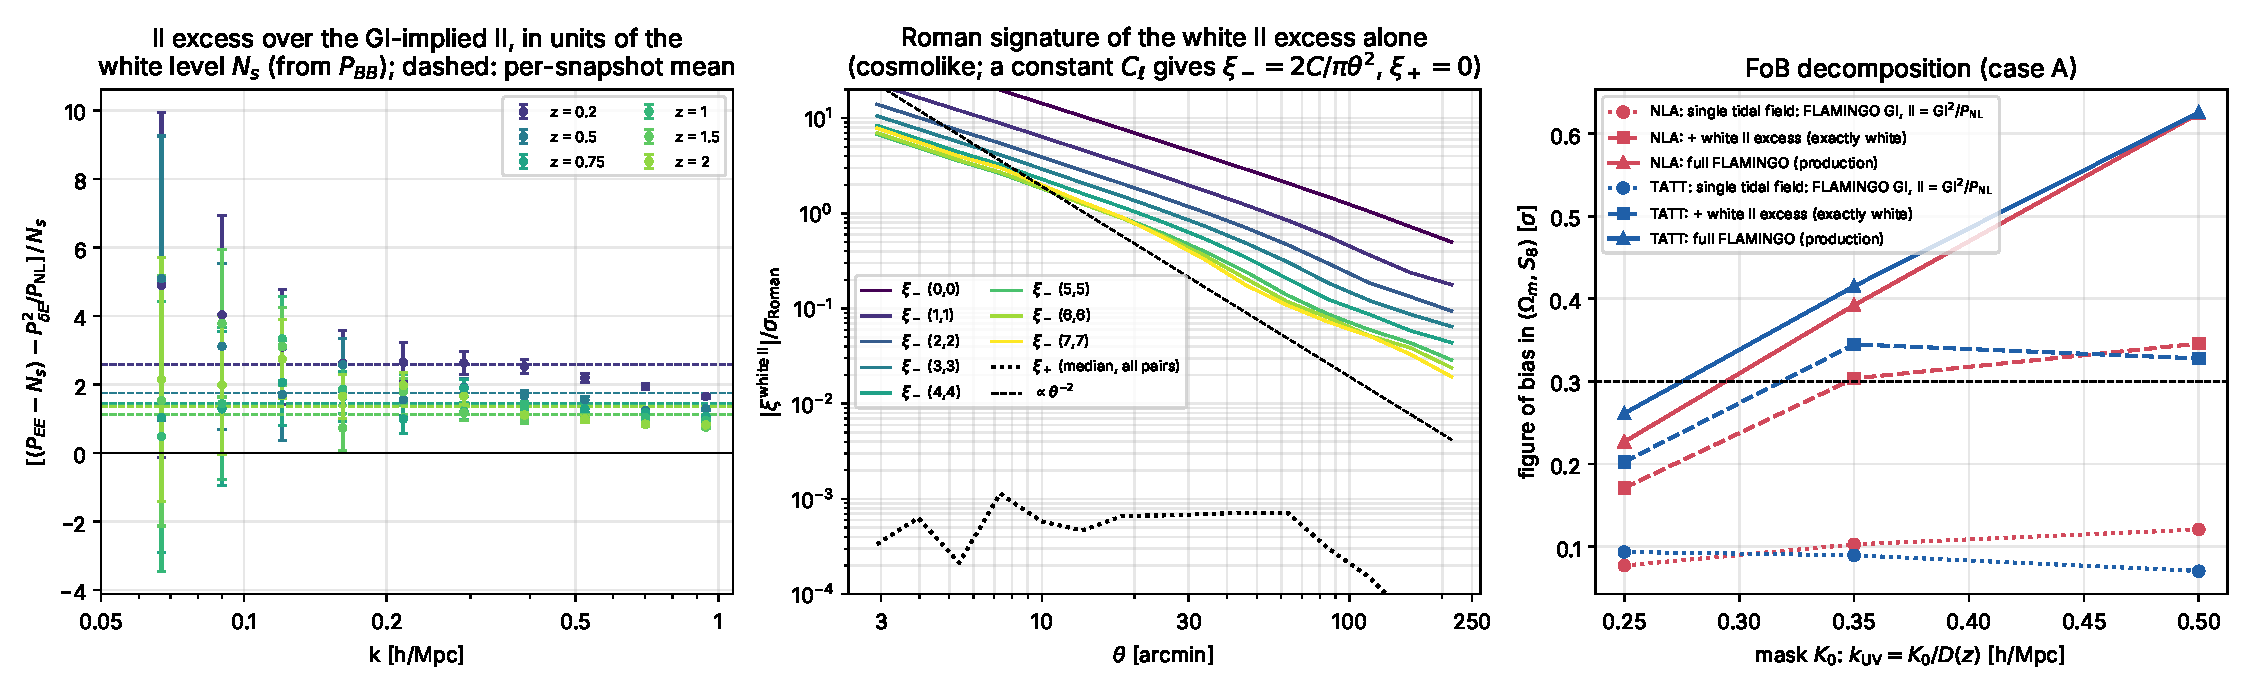
\includegraphics[width=\textwidth]{fig_white_ii.pdf}
\caption{Left: $X(k)/N_s$. Middle: Roman $\xi_\pm/\sigma$ of the white term alone. Right: FoB decomposition.}\label{fig:white}\end{figure}

\section{$\dchi_{\rm FL}\rightarrow\dchi_{\rm Roman}$}\label{sec:translate}
With $u$ the residual (model minus FLAMINGO) in units of FLAMINGO's error per cell (snapshot $s$, spectrum $X\in\{\delta E,EE\}$, node $k_i$), the two metrics are
\begin{equation}
\dchi_{\rm FL}=u^{\rm T}u,\qquad \dchi_{\rm Roman}=u^{\rm T}\mathsf{A}\,u,\qquad \mathsf{A}=\mathsf{S}\,\mathsf{J}^{\rm T}\mathsf{C}^{-1}\mathsf{J}\,\mathsf{S},
\end{equation}
where $\mathsf{J}=\partial\xi_\pm/\partial P_{X}(k_i,z_s)$ is computed with cosmolike one cell at a time (unit hat in $\ln k$ through \texttt{sim\_IA}), $\mathsf{C}$ is the Gaussian $\xi_\pm$ covariance on the mask and $\mathsf{S}={\rm diag}(\sigma_{\rm FL})$. $\mathrm{diag}(\mathsf{A})$ is the Roman $\dchi$ per unit FLAMINGO $\chi^2$ placed in one cell; summed over the 26 cells at each $k$ (mask $0.35/D$):
\begin{center}\small
\begin{tabular}{l*{11}{c}}
\toprule
$k$ & 0.067 & 0.09 & 0.12 & 0.16 & 0.22 & 0.29 & 0.39 & 0.52 & 0.70 & 0.94 & $>2$\\
weight & 0.19 & 0.26 & 0.18 & 0.11 & 0.065 & 0.035 & 0.020 & 0.010 & 0.0035 & 0.0015 & $<2\!\times\!10^{-4}$\\
\bottomrule
\end{tabular}
\end{center}
90\% of the weight is at $k\le0.22$, 97\% at $k\le0.39$, and $z=0.75$--$2$ carry 80\% of it. $\dchi_{\rm Roman}=1$ therefore corresponds to $\dchi_{\rm FL}\simeq20$--$100$ for a misfit at $k\le0.15$ and $z=0.75$--$2$, $300$--$1000$ at $k\simeq0.4$--$0.5$, and $>10^4$ at $k>1$. For the actual NLA/TATT residuals the ratio is 0.02--0.04 for fits with $k_{\max}\le0.22$, 0.01 at 0.29, 0.005 at 0.4--0.7 and $10^{-3}$ above 1 (Fig.~\ref{fig:tr}). The eigen-decomposition of $\mathsf{A}$ gives the extremes: an amplitude-like residual needs $\dchi_{\rm FL}\simeq700$ for Roman 1; the worst direction (a large-scale GI/II residual at $z=1$--2, poorly constrained by the box) needs only $\simeq10$.

\begin{figure}[H]\centering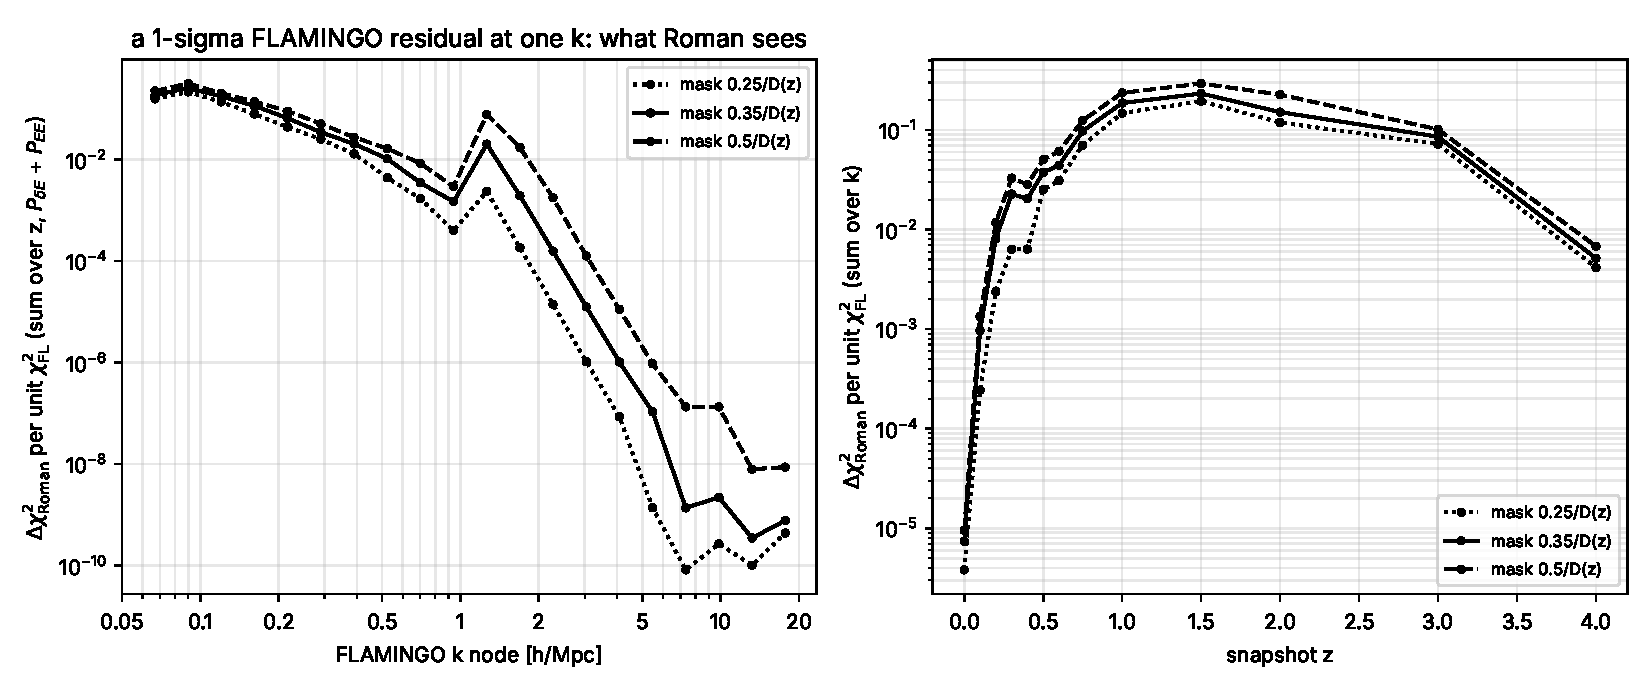
\includegraphics[width=\textwidth]{fig_kmax_weight.pdf}
\caption{Roman $\dchi$ per unit FLAMINGO $\chi^2$, per $k$ node (left) and per snapshot (right), three masks.}\end{figure}
\begin{figure}[H]\centering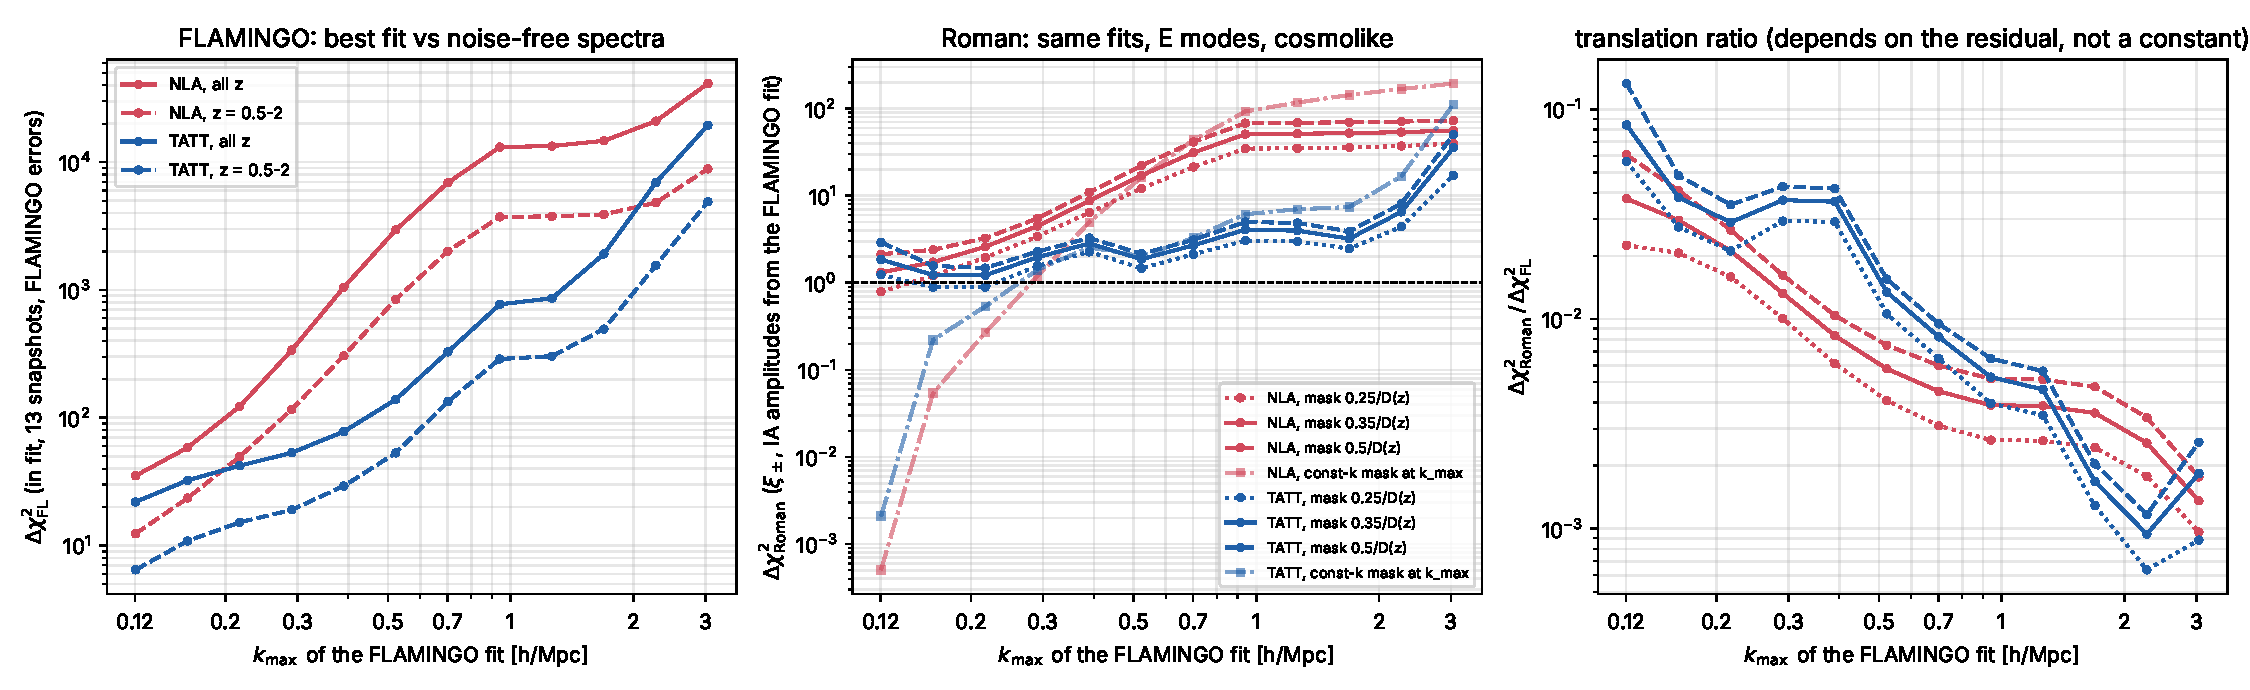
\includegraphics[width=\textwidth]{fig_kmax_dchi2.pdf}
\caption{Left: $\dchi_{\rm FL}$ of the v2 fits (free $N_s$) versus $k_{\max}$. Middle: Roman $\dchi$ of the same fits (IA amplitudes from FLAMINGO, E modes, cosmolike). Right: their ratio.}\label{fig:tr}\end{figure}

\section{Roman: figure of bias and scale cuts}\label{sec:roman}
Data vector: $\xi_\pm$ (8 bins, 15 angular bins 2.5--250$'$, 1080 points) $=\xi_{GG}({\rm D3A})+\xi_{\rm IA}({\rm FLAMINGO})$, the FLAMINGO $P_{\delta E},P_{EE}$ injected through cosmolike's \texttt{sim\_IA} tables (no trimming; ratios to $P_{\rm NL}$ held outside the measured range). Gaussian covariance (2415~deg$^2$, 41.3/8 gal/arcmin$^2$ per bin, $\sigma_e=0.30$). Masks: IR/UV with $\alpha=0.05$ on GG plus an NLA baseline, as \texttt{make\_uv\_scale\_cuts.py}, for $k_{\rm UV}=K_0/D(z)$ (production) and for the $z$-dependent cuts of Sec.~\ref{sec:gof} scaled by a factor $f$. Fit: IA parameters exact (cosmolike), cosmology through its linear response refreshed at the IA solution, trust-region least squares with the IA bounded to the chain priors; checked against fully non-linear fits (identical to all quoted digits). Figure of bias from the Fisher matrix at the solution (IA marginalised with the flat-prior width),
\begin{equation}
{\rm FoB}=\sqrt{\delta\theta^{\rm T}\,\Sigma_\theta^{-1}\,\delta\theta},\qquad \theta=(\Omega_m,S_8),\qquad
\sigma^2_{\rm FoB}=g^{\rm T}\,\mathsf{B}\,\mathsf{J}\mathsf{S}\mathsf{S}\mathsf{J}^{\rm T}\mathsf{B}^{\rm T}g\ \ (\text{FLAMINGO noise}),
\end{equation}
with $\mathsf{B}$ the linear estimator of the shift and $g=\Sigma_\theta^{-1}\delta\theta/{\rm FoB}$.

\begin{table}[H]\centering\small
\begin{tabular}{l|cc|cc}
\toprule
mask $K_0$ ($k_{\rm UV}=K_0/D$) & NLA $\chi^2$ & NLA FoB & TATT $\chi^2$ & TATT FoB\\
\midrule
0.2 & 0.44 & $0.24\pm0.07$ & 0.37 & $0.23\pm0.06$\\
0.25 & 0.81 & $0.23\pm0.07$ & 0.68 & $0.26\pm0.06$\\
0.3 & 1.18 & $0.31\pm0.08$ & 0.96 & $0.34\pm0.05$\\
0.35 & 1.48 & $0.39\pm0.09$ & 1.25 & $0.42\pm0.07$\\
0.4 & 1.90 & $0.61\pm0.09$ & 1.55 & $0.58\pm0.06$\\
0.5 & 2.53 & $0.62\pm0.11$ & 2.06 & $0.63\pm0.09$\\
0.6 & 3.38 & $0.80\pm0.13$ & 2.70 & $0.76\pm0.10$\\
\bottomrule
\end{tabular}
\caption{Production mask family, case A ($\Omega_m$, $A_s$ free). With FLAMINGO's $P_{BB}$ added to the data: 0.22/0.25 at $0.35/D$; raw instead of smoothed spectra: 0.53/0.50. With one free white II amplitude: 0.16/0.12 at $0.35/D$, 0.44/0.28 at $0.5/D$.}
\end{table}

\begin{figure}[H]\centering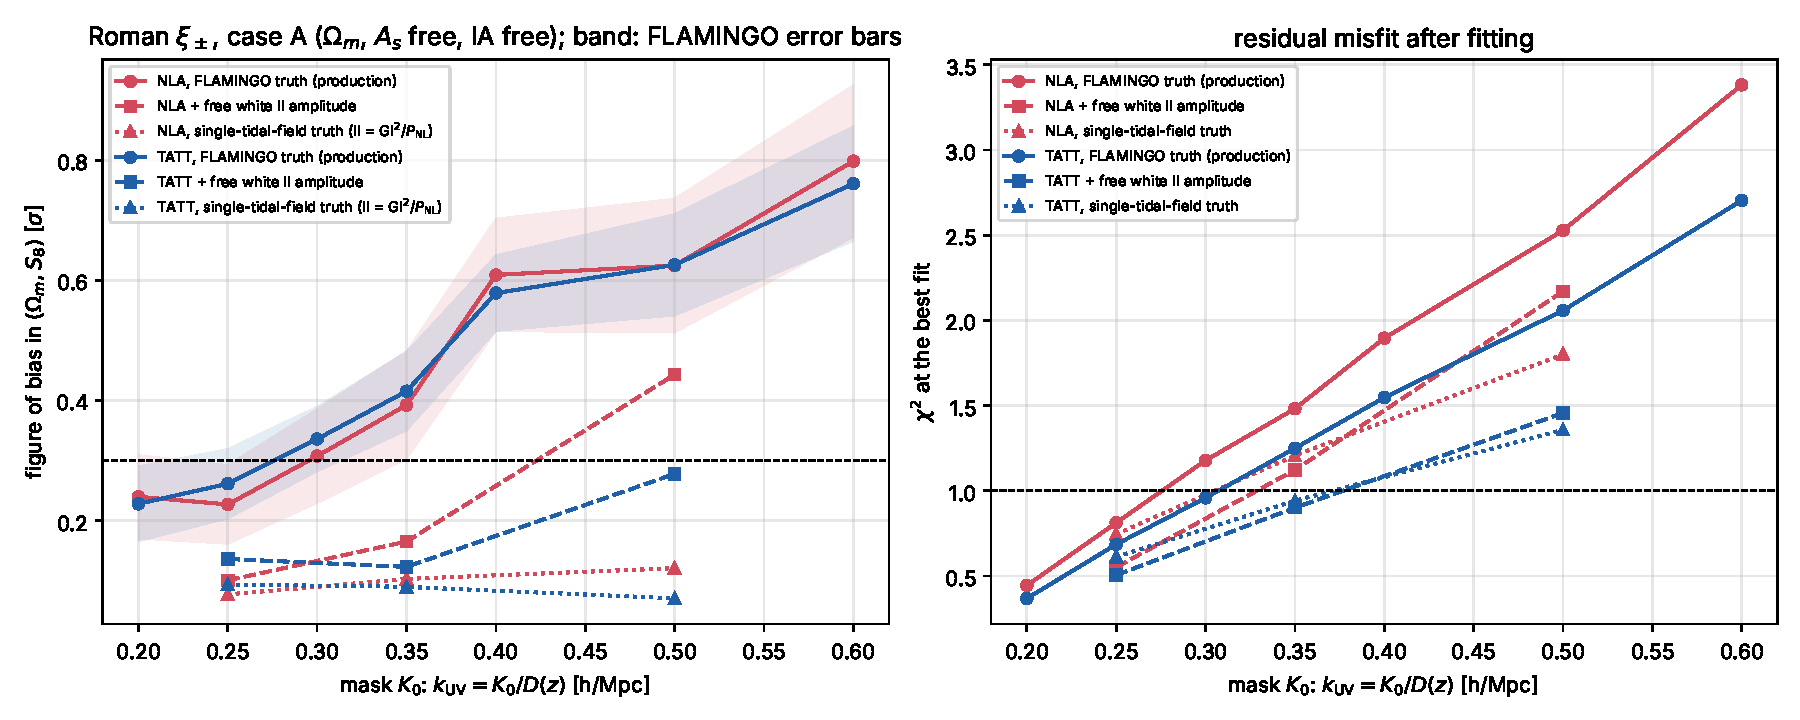
\includegraphics[width=\textwidth]{fig_kmax_fob.pdf}
\caption{FoB and residual $\chi^2$ versus $K_0$: production truth, with a free white II amplitude, and the single-tidal-field truth.}\end{figure}

\begin{table}[H]\centering\small
\begin{tabular}{llrr|rr|rrr|rrr}
\toprule
cut shape & $f$ & $k_{\rm UV}(0.5)$ & $k_{\rm UV}(1)$ & pts & & $\dchi_{\rm NLA}$ & NLA $\chi^2$ & FoB & $\dchi_{\rm TATT}$ & TATT $\chi^2$ & FoB\\
\midrule
NLA GoF & 1 & 0.092 & 0.120 & 9 && 0.00 & 0.00 & 0.01 & 0.00 & 0.00 & 0.01\\
NLA GoF & 2 & 0.184 & 0.241 & 48 && 0.34 & 0.16 & 0.08 & 0.44 & 0.10 & 0.13\\
NLA GoF & 2.8 & 0.257 & 0.337 & 115 && 1.65 & 0.41 & 0.12 & 2.49 & 0.31 & 0.14\\
NLA GoF & 4 & 0.367 & 0.481 & 305 && 10.1 & 1.21 & 0.32 & 17.9 & 0.91 & 0.35\\
TATT GoF & 0.7 & 0.199 & 0.204 & 63 && 0.22 & 0.04 & 0.06 & 0.14 & 0.01 & 0.05\\
TATT GoF & 1 & 0.285 & 0.291 & 145 && 1.51 & 0.22 & $0.23\pm0.09$ & 0.98 & 0.19 & $0.22\pm0.09$\\
TATT GoF & 1.4 & 0.399 & 0.407 & 237 && 11.5 & 0.76 & 0.33 & 7.0 & 0.70 & 0.34\\
TATT GoF & 2 & 0.569 & 0.581 & 313 && 27.8 & 1.59 & 0.51 & 23.0 & 1.35 & 0.49\\
TATT GoF & 2.8 & 0.797 & 0.814 & 384 && 59.3 & 2.83 & 0.90 & 59.2 & 2.34 & 0.79\\
\bottomrule
\end{tabular}
\caption{$z$-dependent masks from the simulation cuts. $\dchi$: FLAMINGO versus the model with the FLAMINGO-fitted amplitudes at $k_{\max}=f\times{\rm cut}(z)$, no Roman refit; $\chi^2$ and FoB: IA and cosmology refitted in Roman. With the white template at $f=2$ (TATT shape): FoB 0.35 (NLA), 0.19 (TATT).}\label{tab:roman}
\end{table}

\begin{figure}[H]\centering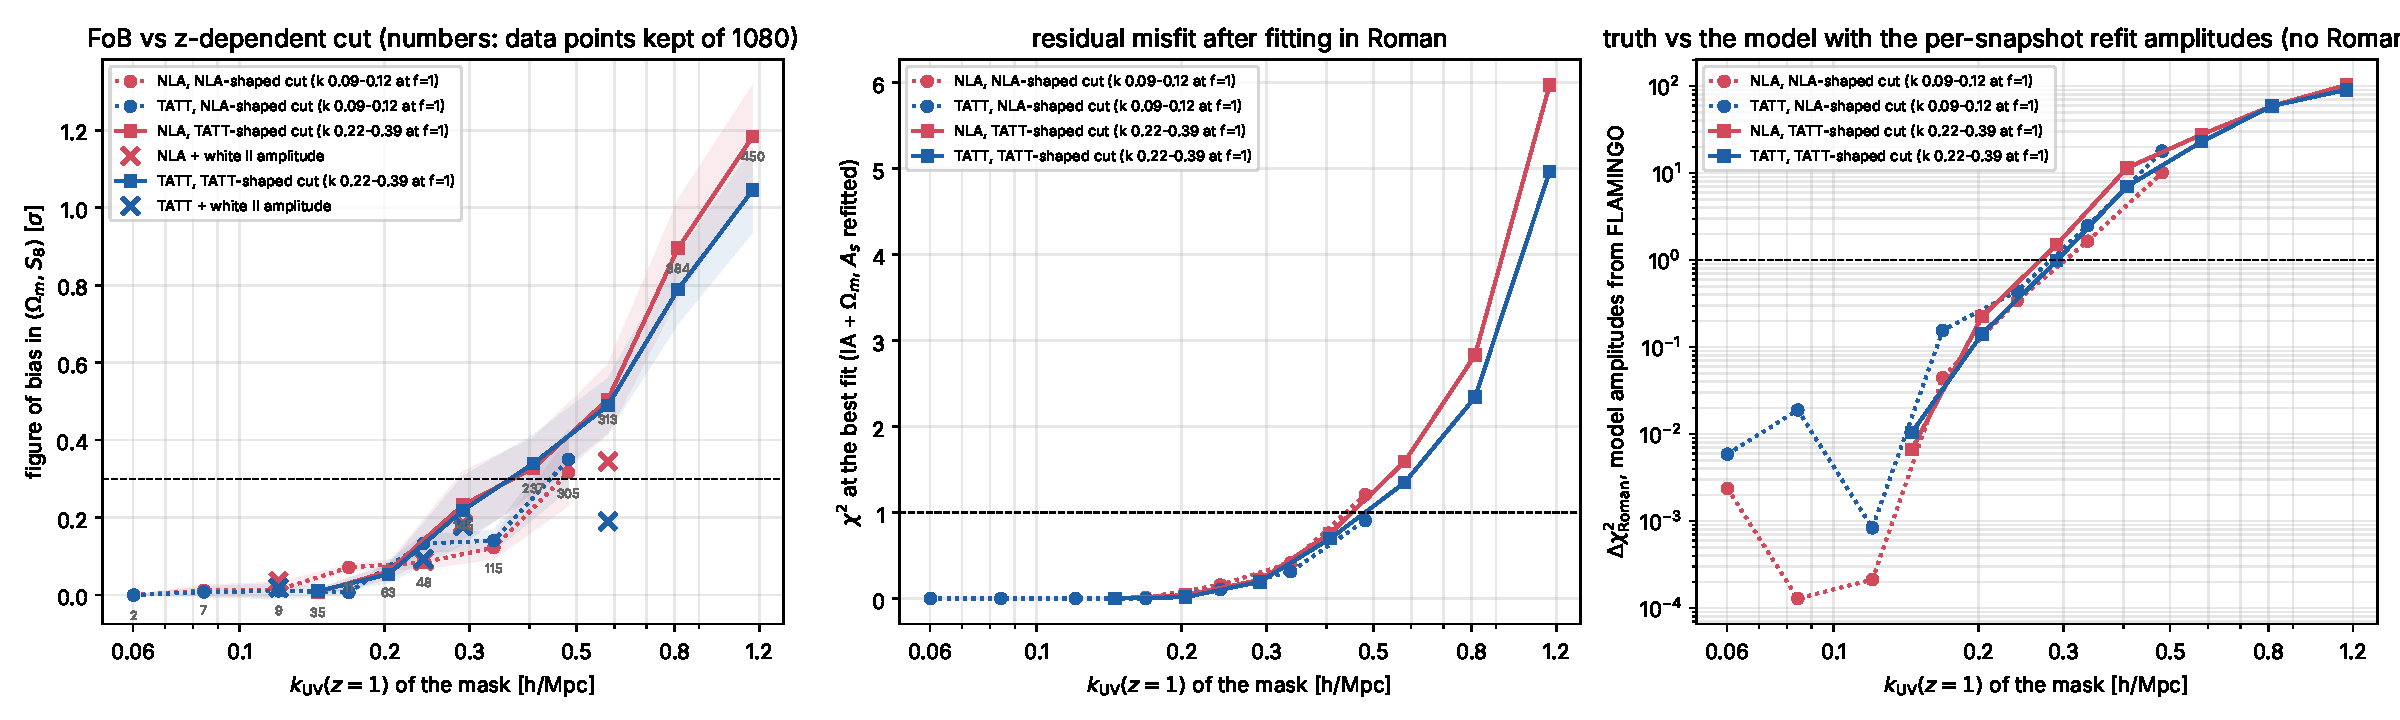
\includegraphics[width=\textwidth]{fig_v3_roman.pdf}
\caption{Roman versus the $z$-dependent cuts (horizontal axis: $k_{\rm UV}$ at $z=1$).}\end{figure}

\section{The Roman test: all parameters free, with controls}\label{sec:romantest}
The quantity the chain measures is the shift of the cosmology when the model is fitted with every parameter free and the chain priors, so that is the test (\texttt{v3/roman\_test.py}). For each mask, model and cosmology setting (A: $\Omega_m,A_s$; B: $\Omega_m,A_s,n_s,H_0,\Omega_b$ with Gaussian priors of the width of the chain's flat priors) all parameters are fitted to the FLAMINGO-injected $\xi_\pm$, and the FoB (IA marginalised with the flat-prior width), its truth-noise uncertainty and $\chi^2$ at the best fit are recorded. Three controls run at every mask and case: TATT on the Part~1a TATT truth (matched model), NLA on that truth (the Part~1 mismodelling bias), and NLA on an NLA truth pushed through the same \texttt{sim\_IA} tables as FLAMINGO (injection path). Fig.~\ref{fig:romantest}, Table~\ref{tab:romantest}, \texttt{v3/roman\_test.csv}.

\begin{figure}[H]\centering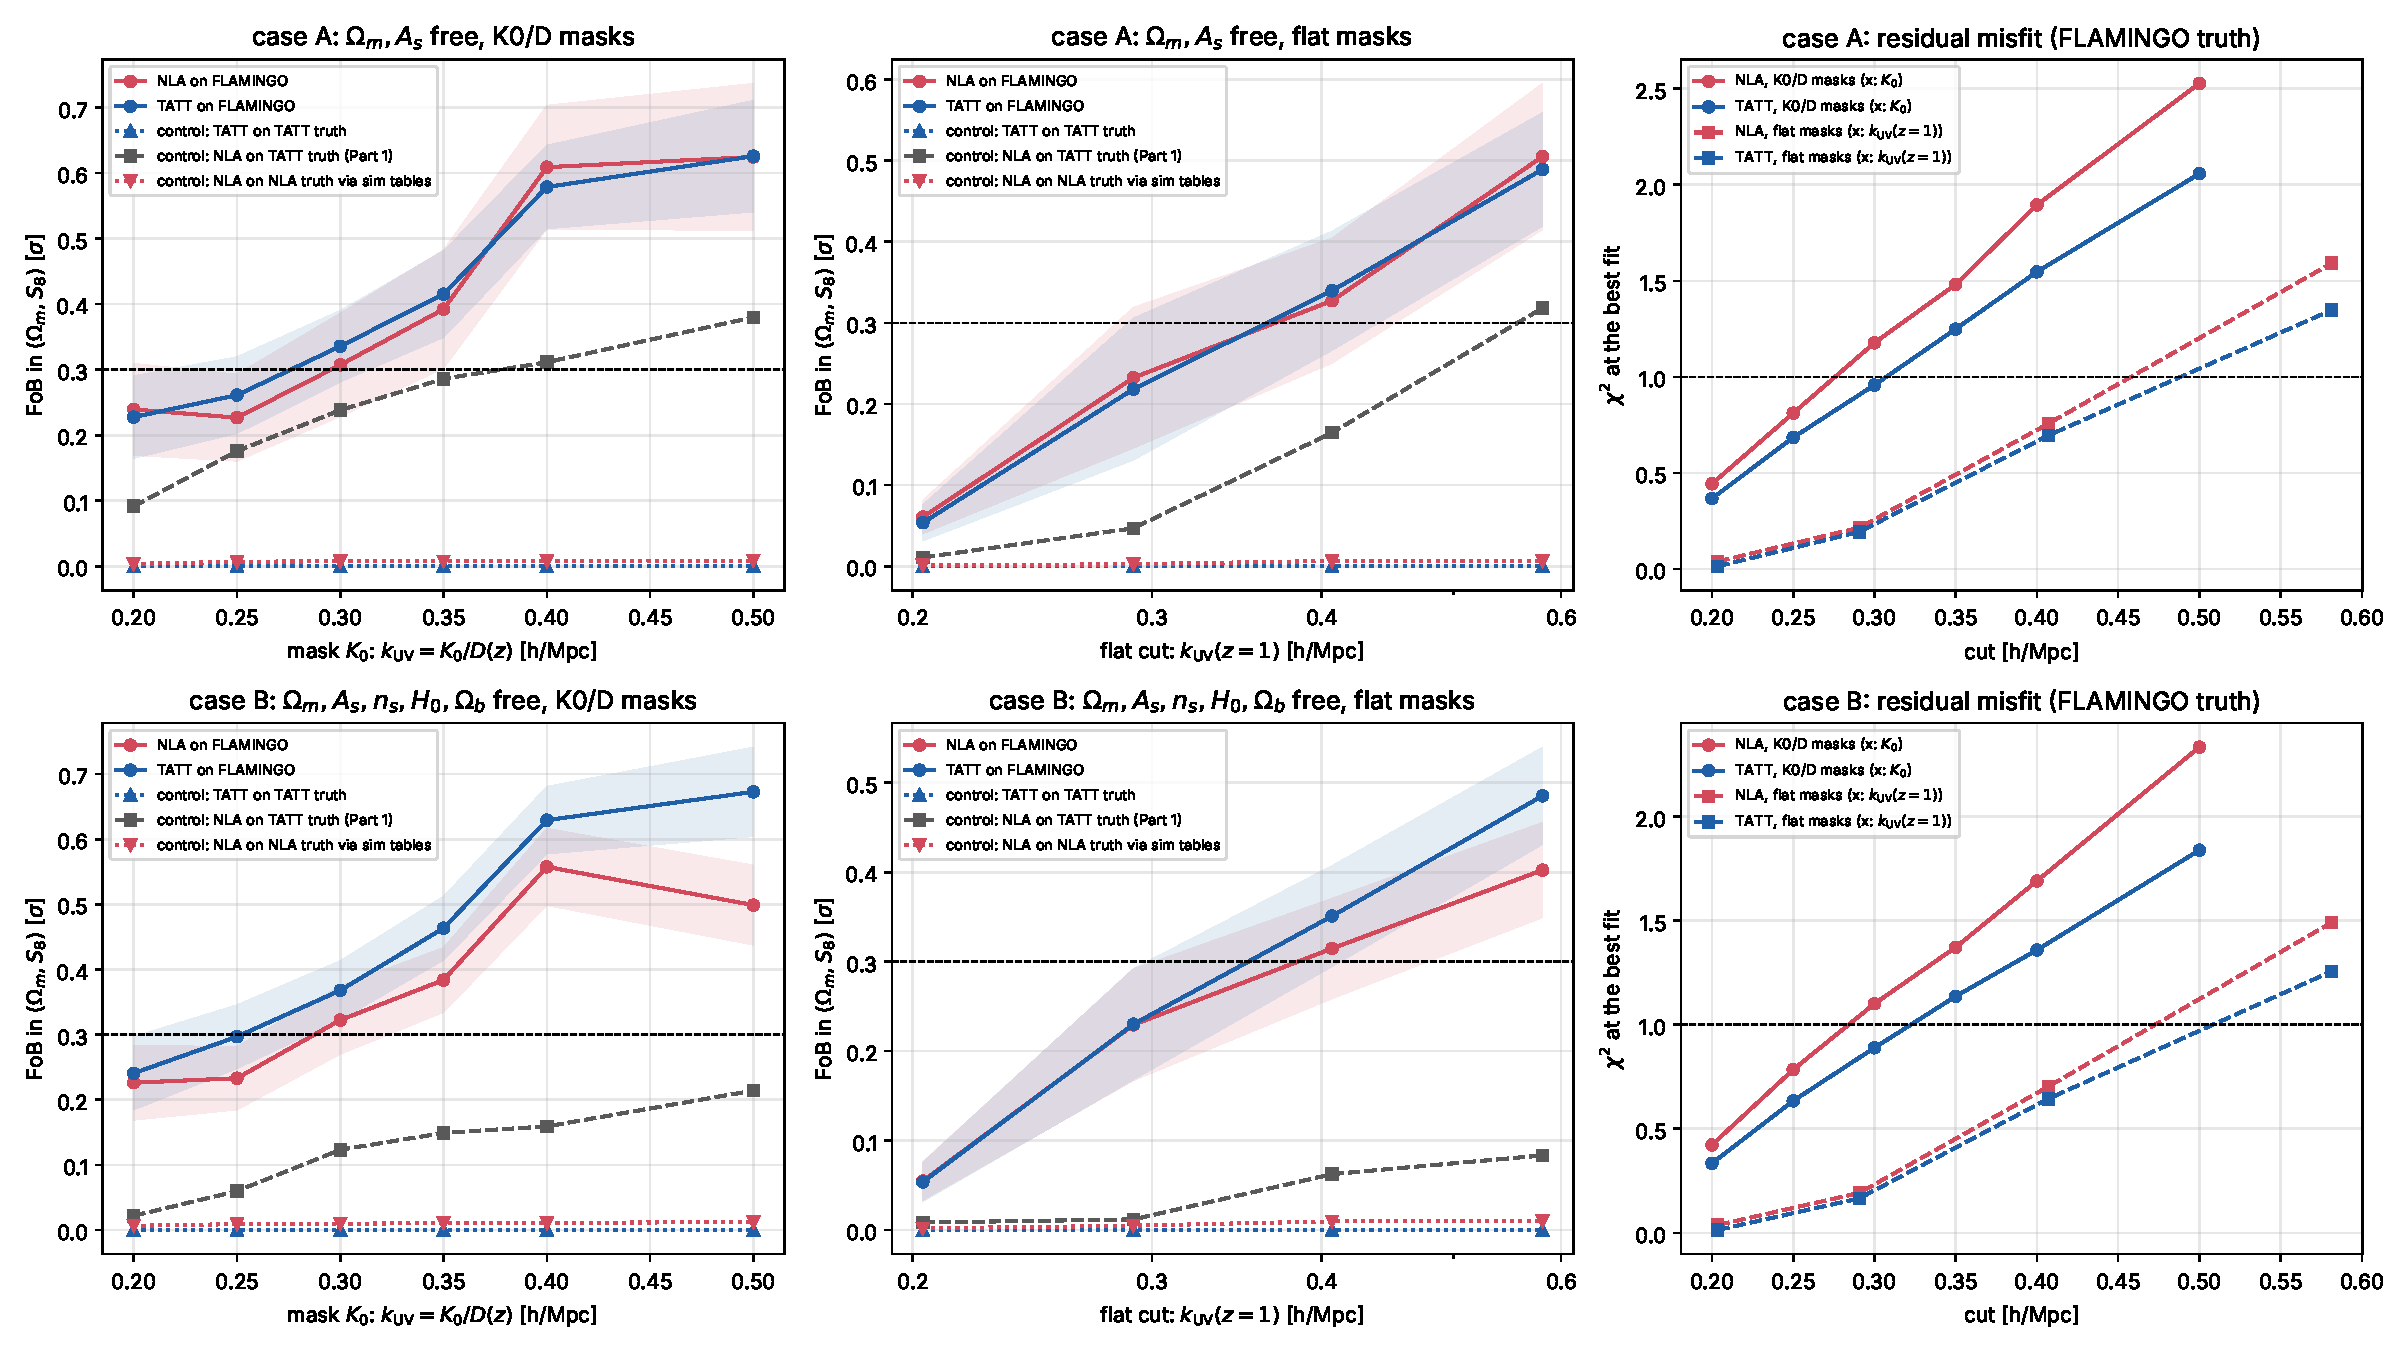
\includegraphics[width=\textwidth]{fig_roman_test.pdf}
\caption{FoB (left, middle; band: FLAMINGO error bars) and best-fit $\chi^2$ (right) versus cut, for the production $K_0/D(z)$ masks and the flat $z$-dependent masks, cases A (top) and B (bottom), with the three controls.}\label{fig:romantest}\end{figure}

\begin{table}[H]\centering\footnotesize\setlength{\tabcolsep}{4pt}
\begin{tabular}{l|cc|cc|cc|ccc}
\toprule
 & \multicolumn{2}{c|}{NLA on FLAMINGO} & \multicolumn{2}{c|}{TATT on FLAMINGO} & \multicolumn{2}{c|}{case B FoB} & \multicolumn{3}{c}{controls (case A FoB)}\\
mask & $\chi^2$ & FoB (A) & $\chi^2$ & FoB (A) & NLA & TATT & TATT/TATT & NLA/TATT & NLA/NLA inj.\\
\midrule
$K_0/D$ 0.2 & 0.44 & $0.24\pm0.07$ & 0.37 & $0.23\pm0.06$ & 0.23 & 0.24 & 0.000 & 0.09 & 0.004\\
$K_0/D$ 0.25 & 0.81 & $0.23\pm0.07$ & 0.69 & $0.26\pm0.06$ & 0.23 & 0.30 & 0.000 & 0.18 & 0.007\\
$K_0/D$ 0.3 & 1.18 & $0.31\pm0.08$ & 0.96 & $0.34\pm0.06$ & 0.32 & 0.37 & 0.000 & 0.24 & 0.008\\
$K_0/D$ 0.35 & 1.48 & $0.39\pm0.09$ & 1.25 & $0.42\pm0.07$ & 0.38 & 0.46 & 0.000 & 0.29 & 0.008\\
$K_0/D$ 0.4 & 1.90 & $0.61\pm0.09$ & 1.55 & $0.58\pm0.06$ & 0.56 & 0.63 & 0.000 & 0.31 & 0.008\\
$K_0/D$ 0.5 & 2.53 & $0.63\pm0.11$ & 2.06 & $0.63\pm0.09$ & 0.50 & 0.67 & 0.000 & 0.38 & 0.009\\
\midrule
flat 0.20 & 0.04 & $0.06\pm0.02$ & 0.01 & $0.05\pm0.02$ & 0.06 & 0.05 & 0.000 & 0.01 & 0.01\\
flat 0.29 & 0.22 & $0.23\pm0.09$ & 0.19 & $0.22\pm0.09$ & 0.23 & 0.23 & 0.000 & 0.05 & 0.01\\
flat 0.41 & 0.76 & $0.33\pm0.08$ & 0.70 & $0.34\pm0.07$ & 0.32 & 0.35 & 0.000 & 0.17 & 0.01\\
flat 0.58 & 1.59 & $0.51\pm0.09$ & 1.35 & $0.49\pm0.07$ & 0.40 & 0.49 & 0.000 & 0.32 & 0.01\\
\bottomrule
\end{tabular}
\caption{The Roman test. ``flat $k$'': the TATT-shaped $z$-dependent mask, labelled by $k_{\rm UV}(z=1)$ in $h$/Mpc. The matched-model control is zero to three decimals and the injection control below 0.01 everywhere, so every nonzero FoB is model mismatch. The NLA-on-TATT control is the Part~1 bias of the Part~1a fiducial.}\label{tab:romantest}
\end{table}

\paragraph{Reading.} Cases A and B agree to $\pm0.05$: freeing $n_s$, $H_0$, $\Omega_b$ does not let either model absorb the residual. FoB $=0.3$ is crossed at $K_0\simeq0.3$ or $k_{\rm UV}(z=1)\simeq0.37$ for both models in both cases, and $\chi^2$ at the best fit reaches 1 at about the same place ($K_0\simeq0.3$ for NLA, $0.32$ for TATT; flat $0.47$ and $0.50$). The simulation's TATT cut (flat 0.29, 145 points) gives FoB $0.22$--$0.23\pm0.09$ and $\chi^2\simeq0.2$ for either model. The Part~1 control shows that NLA fitted to the Part~1a TATT fiducial stays below $0.3\sigma$ up to $K_0=0.35$ in case A (0.29) and everywhere in case B ($\le0.21$).

\paragraph{MCMC check (\texttt{v3/roman\_mcmc.py}).} At $K_0=0.3/D$, case A, emcee over ($\Omega_m$, $A_s$, IA) with the IA exact and the cosmology linearised at the MAP IA, flat chain priors, 16 walkers, 600 steps (autocorrelation 30--70 steps, so the posterior means carry a sampling uncertainty of about $0.1\sigma$):
\begin{center}\small
\begin{tabular}{l|cc|cc|cc}
\toprule
 & \multicolumn{2}{c|}{$\Delta S_8/\sigma$} & \multicolumn{2}{c|}{$\Delta\Omega_m/\sigma$} & \multicolumn{2}{c}{FoB (posterior cov.)}\\
run & MAP & posterior mean & MAP & posterior mean & MAP & posterior mean\\
\midrule
TATT on FLAMINGO & $+0.28$ & $+0.28$ & $-0.03$ & $-0.23$ & 0.30 & 0.43\\
TATT on TATT (matched control) & $0.00$ & $+0.24$ & $0.00$ & $+0.06$ & 0.00 & 0.24\\
NLA on FLAMINGO & $+0.30$ & $+0.18$ & $+0.07$ & $-0.13$ & 0.30 & 0.25\\
\bottomrule
\end{tabular}
\end{center}
The MAP shifts of the linearised fits are reproduced (the Fisher FoB of 0.34 for TATT becomes 0.30 with the posterior covariance). The matched TATT control, which has zero MAP shift, has a posterior-mean shift of $0.24\sigma$: the prior-volume (projection) effect of the weakly constrained $\eta_2$ and $b_{\rm TA}$ ($b_{\rm TA}$ posterior mean 0.41 against a truth of 0.18; $A_2$ $-0.80\pm0.67$ against $-1.08$). The TATT-on-FLAMINGO posterior mean therefore mixes mismodelling ($\simeq0.3\sigma$) with a projection shift of comparable size, and the paper should quote MAP shifts, or posterior means with the matched-model run subtracted, as the Part~1 plan already prescribes. NLA has no such effect within the sampling noise.

\paragraph{Still open for the paper.} The covariance here is Gaussian; the production covariance (non-Gaussian and super-sample terms) lowers both the FoB in $\sigma$ units and the weight of the small angles that carry the residual, so the crossing point should be recomputed with it. And the chains should be repeated with the cocoa likelihood at the one or two masks finally chosen.

\section{How $k_{\rm UV}$ depends on redshift}\label{sec:kuvz}
The production masks assume $k_{\rm UV}(z)=K_0/D(z)$, the scaling of the nonlinear scale in perturbation theory: for $K_0=0.2$, $k_{\rm UV}=0.22,\,0.26,\,0.33,\,0.40,\,0.48\hmpc$ at $z=0.2,\,0.5,\,1,\,1.5,\,2$ ($D=0.90,\,0.77,\,0.61,\,0.50,\,0.42$), a factor 2.2 across the core. The cuts measured in FLAMINGO are nearly flat in $z$ (Fig.~\ref{fig:kuvz}): the TATT GoF cut is 0.22 at $z\le0.4$, 0.29 at $z=0.5$--$1.5$ and 0.39 at $z=2$ (a factor 1.3 at most); the NLA GoF cut scatters between 0.09 and 0.12 with no trend; the anchored, 5\%-GI and 10\% criteria behave the same way. No single $K_0/D(z)$ curve follows the measured points: $K_0=0.15$ matches TATT at $z\simeq0.5$--$2$ but is too tight at $z=0.2$ (0.17 against 0.22); $K_0=0.2$ matches at $z=0.2$ but reaches 0.48 at $z=2$. The reading is that the breakdown of both models is governed by the one-halo IA terms (the white II excess and the one-halo GI), whose scale is set by halo sizes and barely evolves, rather than by $k_{\rm NL}(z)$. For the Roman masks of Table~\ref{tab:roman} the measured cut is interpolated in $\ln k$ between the core snapshots and held flat outside them (dotted lines in Fig.~\ref{fig:kuvz}); at $f=1$ the TATT shape is $k_{\rm UV}=0.285$ at $z=0.5$ and $0.291$ at $z=1$, in effect a constant-$k$ cut. If the $K_0/D(z)$ family is kept for continuity with Part~1, the simulation points to $K_0\simeq0.15$--$0.2$, tighter than needed at low $z$ and looser than measured at $z=1.5$--$2$.

\begin{figure}[H]\centering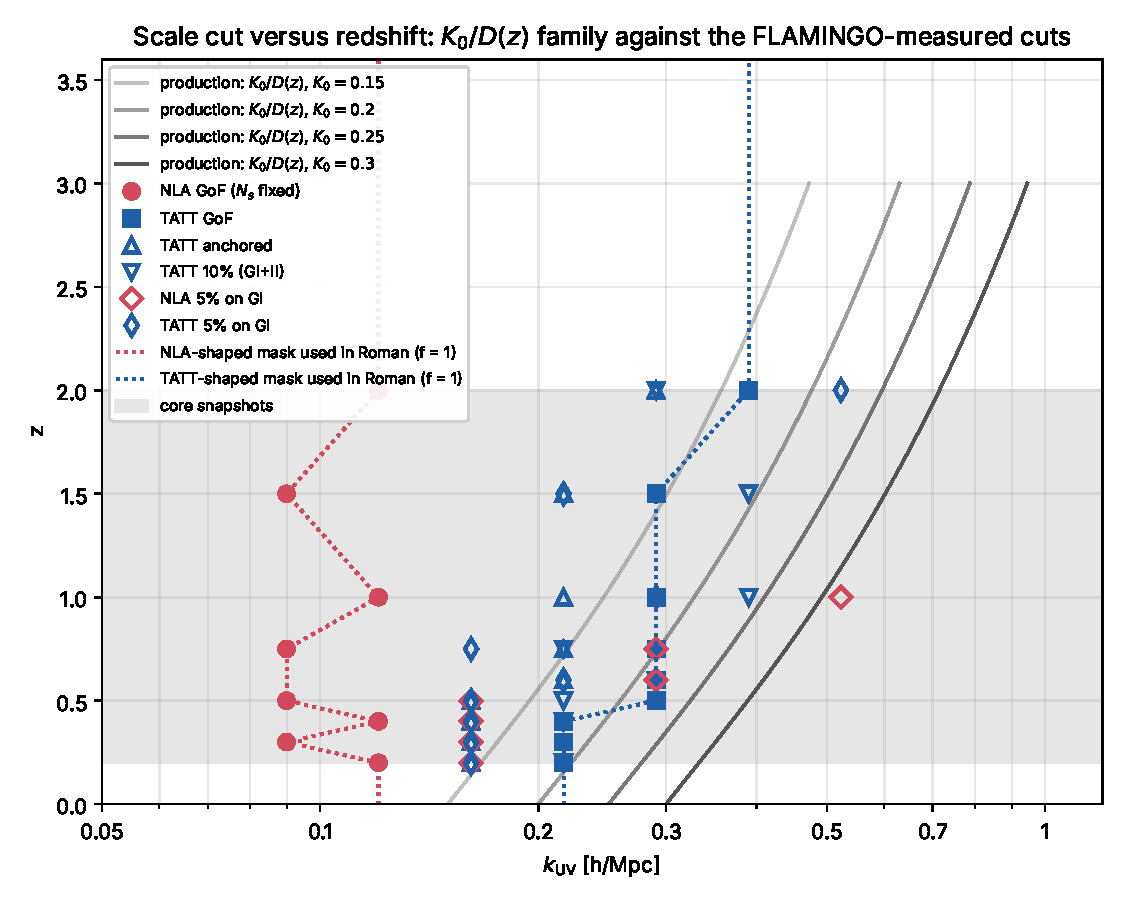
\includegraphics[width=0.8\textwidth]{fig_kuv_z.pdf}
\caption{$k_{\rm UV}$ versus $z$ ($k$ horizontal, $z$ vertical). Grey curves: $K_0/D(z)$ for $K_0=0.15$--$0.3$. Points: per-snapshot cuts from the six simulation criteria (core snapshots). Dotted: the $z$-dependent masks used in Roman at $f=1$.}\label{fig:kuvz}\end{figure}

\section{The redshift scaling of the cut: $k_{\max}(z)=k_0\,D(z)^{-2/(3+n)}$}\label{sec:knl}
\paragraph{Definitions.} $D(z)$ is the linear growth factor ($D(0)=1$, CAMB at the D3A cosmology). The non-linear scale is defined by the linear dimensionless power,
\begin{equation}
\Delta^2_{\rm lin}(k_{\rm NL},z)\equiv\frac{k_{\rm NL}^3\,P_{\rm lin}(k_{\rm NL},z)}{2\pi^2}=1 .
\label{eq:dnl}
\end{equation}
For a power-law spectrum $P_{\rm lin}\propto k^{n}$, $\Delta^2_{\rm lin}\propto D(z)^2k^{3+n}$, so
\begin{equation}
k_{\rm NL}(z)=k_{\rm NL}(0)\,D(z)^{-p},\qquad p=\frac{2}{3+n}.
\label{eq:knl}
\end{equation}
The $K_0/D(z)$ family of the production masks (Saraivanov et al.\ 2026, their Eq.~10, ``we assume a $k_{\rm UV}/D(\chi)$ scaling of the non-linear scale'') is the case $n=-1$, $p=1$; a constant comoving $k_{\max}$ is $p=0$ ($n\to\infty$); $n=0$ gives $p=2/3$, $n=-2$ gives $p=2$. The effective index $n_{\rm eff}(k)=d\ln P_{\rm lin}/d\ln k$ at $z=0$ is -1.68, -1.93, -1.77, -2.10, -2.30 at $k=0.1,\,0.2,\,0.3,\,0.5,\,1\hmpc$.

\paragraph{Fit.} For each cut criterion the per-snapshot cuts of the core snapshots are fitted with
\begin{equation}
\ln k_{\max}(z_s)=\ln k_0-p\,\ln D(z_s),\qquad \chi^2(p)=\sum_s\frac{[\ln k_{\max}(z_s)-\ln k_0+p\ln D(z_s)]^2}{\sigma_{\ln k}^2},
\end{equation}
with $\sigma_{\ln k}=\tfrac12\ln1.35=0.15$ (half a step of the $k_{\max}$ grid, on which the cuts are quantised) and $k_0$ profiled out analytically; $n=2/p-3$; the $\Delta\chi^2\le1$ interval in $n$ is read off the profile. The same fit to the exact $k_{\rm NL}(z)$ of Eq.~(\ref{eq:dnl}) gives the $n$ that the real $P_{\rm lin}$ shape implies.

\begin{figure}[H]\centering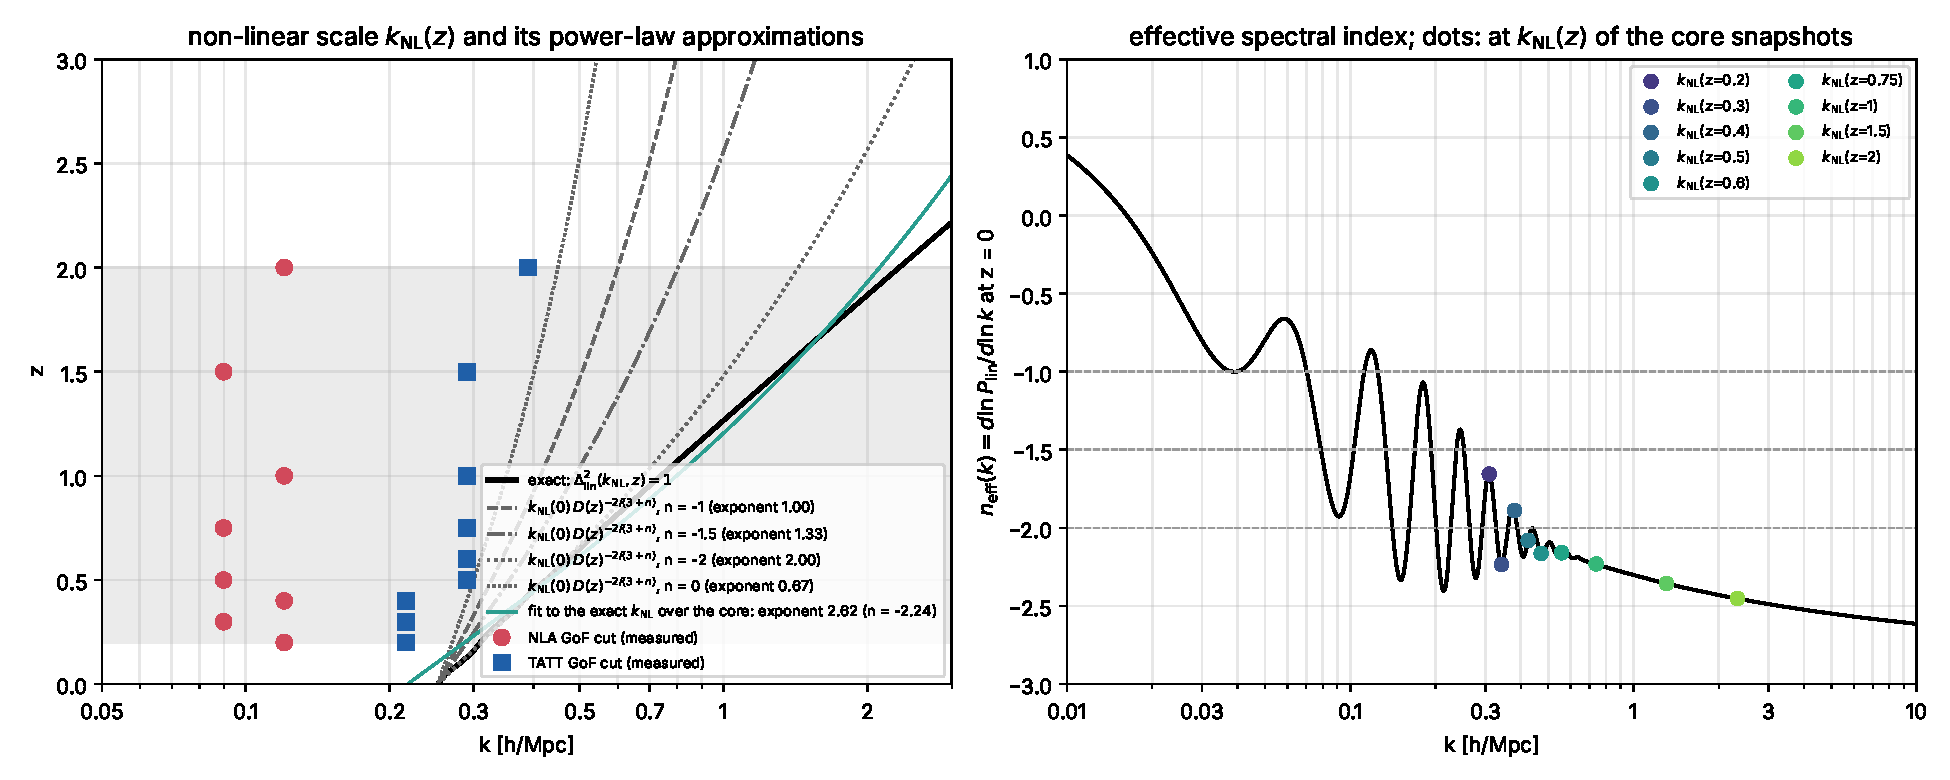
\includegraphics[width=\textwidth]{fig_knl_z.pdf}
\caption{Left: the exact non-linear scale $k_{\rm NL}(z)$ (black) against the power-law approximations $k_{\rm NL}(0)D(z)^{-2/(3+n)}$ for $n=-1$ (the $K_0/D$ family), $-1.5$, $-2$ and $0$, the power-law fit to the exact curve over the core, and the measured NLA and TATT GoF cuts. Right: $n_{\rm eff}(k)$ at $z=0$, with the values at $k_{\rm NL}(z)$ of the core snapshots.}\label{fig:knlz}\end{figure}

\begin{figure}[H]\centering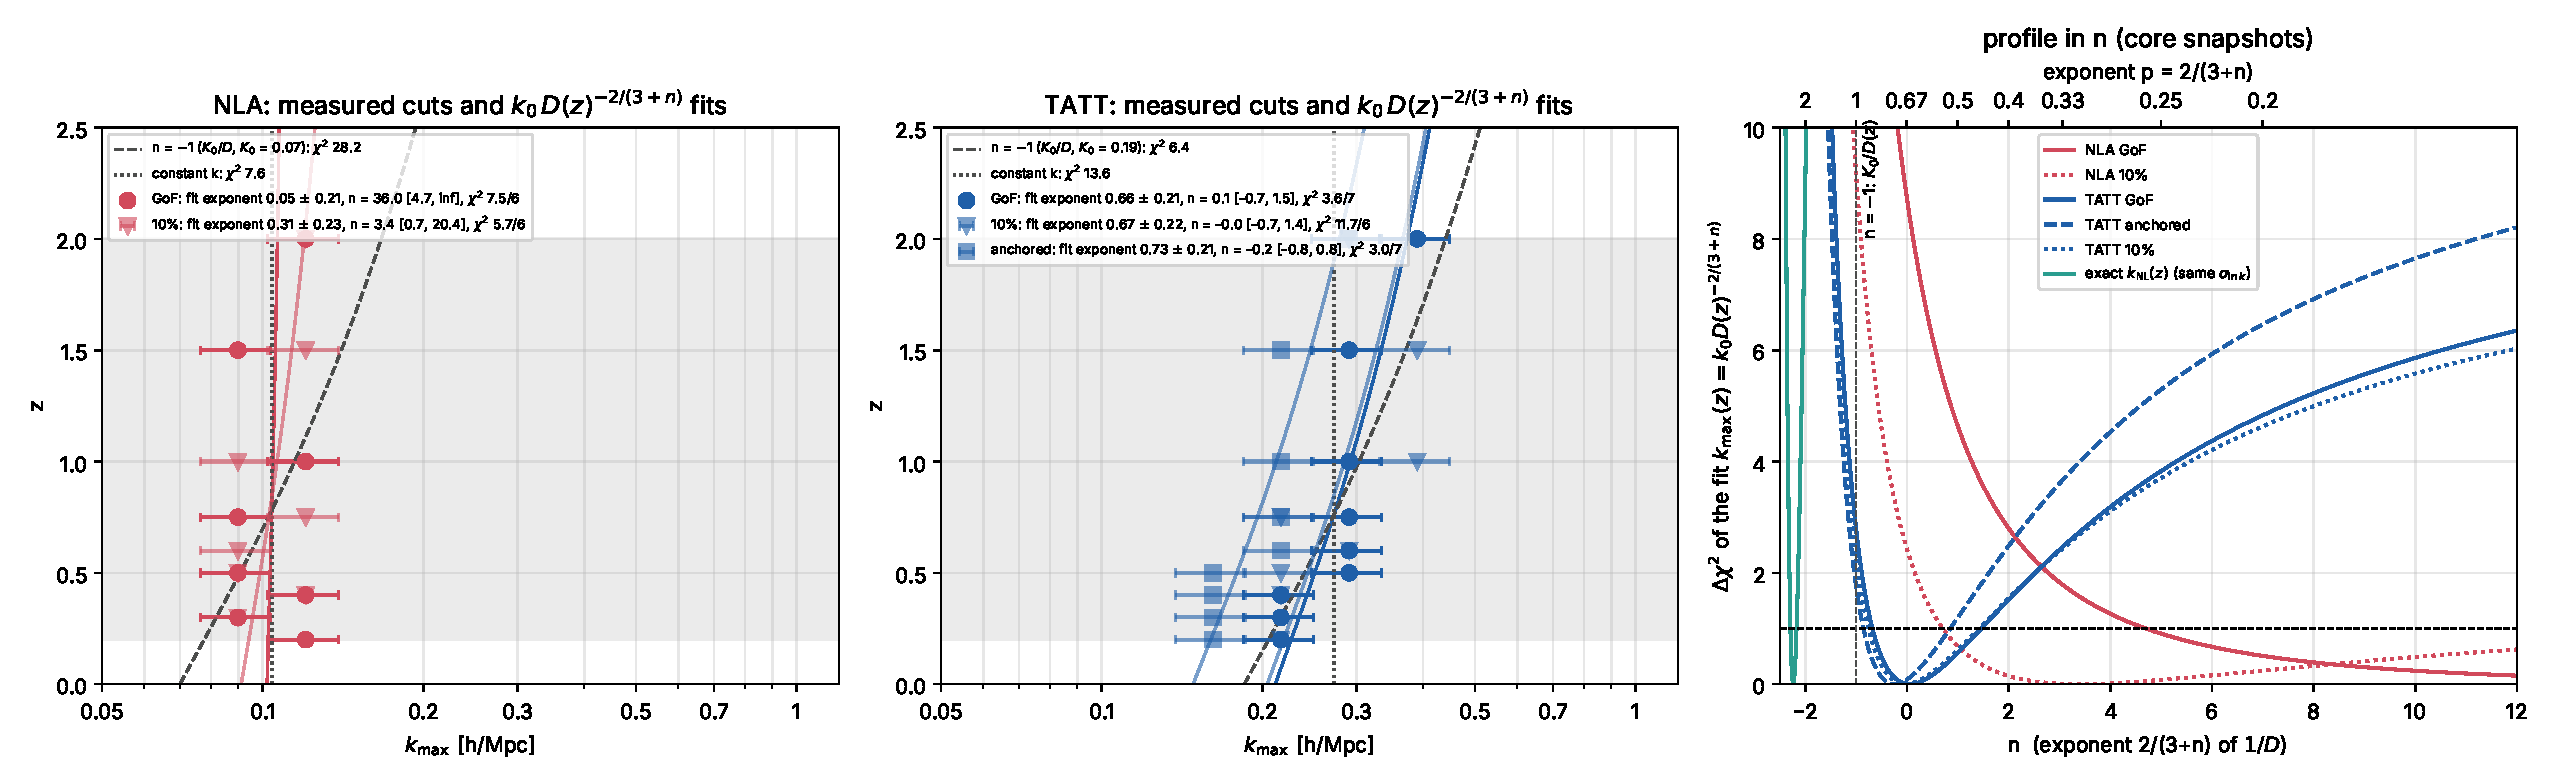
\includegraphics[width=\textwidth]{fig_knl_fit.pdf}
\caption{Left, middle: measured cuts (error bars: half a grid step) with the best-fit $k_0D(z)^{-p}$ curve per criterion, the best $n=-1$ curve (dashed) and the best constant-$k$ cut (dotted), with their $\chi^2$. Right: $\Delta\chi^2$ profiles in $n$ (top axis: the exponent $p$); the dashed vertical line is the $K_0/D(z)$ assumption.}\label{fig:knlfit}\end{figure}

\begin{table}[H]\centering\footnotesize\setlength{\tabcolsep}{4pt}
\caption{Power-law fits $k_{\max}(z)=k_0D(z)^{-p}$, $p=2/(3+n)$, to the measured cuts over the core snapshots ($0.2\le z\le2$), with the $\chi^2$ of the two fixed alternatives. Last rows: the same fit to the stitched-truth GoF cuts (companion PDF) and to the exact $k_{\rm NL}(z)$.}\label{tab:knl}
\resizebox{\textwidth}{!}{%
\begin{tabular}{lcccccc}
\toprule
cut criterion (core snapshots) & $k_0$ & exponent $p$ & $n$ [$\Delta\chi^2\le1$] & $\chi^2$/dof (free $p$) & $\chi^2$ at $n=-1$ & $\chi^2$ constant $k$ \\
\midrule
NLA GoF & 0.102 & 0.05 $\pm$ 0.21 & 36.0 [4.7, $\infty$] & 7.5/6 & 28.2 & 7.6 \\
NLA 10\% & 0.091 & 0.31 $\pm$ 0.23 & 3.4 [0.7, 20.4] & 5.7/6 & 14.8 & 7.6 \\
TATT GoF & 0.211 & 0.66 $\pm$ 0.21 & 0.1 [-0.7, 1.5] & 3.6/7 & 6.4 & 13.6 \\
TATT anchored & 0.148 & 0.73 $\pm$ 0.21 & -0.2 [-0.8, 0.8] & 3.0/7 & 4.8 & 15.4 \\
TATT 10\% & 0.204 & 0.67 $\pm$ 0.22 & -0.0 [-0.7, 1.4] & 11.7/6 & 13.9 & 21.1 \\
\midrule
NLA GoF, stitched truth & 0.216 & 0.69 $\pm$ 0.21 & -0.1 & 15.4 & & \\
TATT GoF, stitched truth & 0.258 & 0.90 $\pm$ 0.21 & -0.8 & 2.4 & & \\
exact $k_{\rm NL}(z)$, $\Delta^2_{\rm lin}=1$ & 0.218 & 2.62 & -2.24 & & & \\
\bottomrule
\end{tabular}}
\end{table}

\paragraph{Reading.}
\begin{itemize}
\item \textbf{The matter non-linear scale grows much faster than $1/D$.} Over the core $k_{\rm NL}$ runs from 0.31 ($z=0.2$) to 0.74 ($z=1$) and 2.3$\hmpc$ ($z=2$), a power-law exponent $p=2.6$ ($n=-2.2$), because $n_{\rm eff}=-1.7$ to $-2.5$ at $k_{\rm NL}(z)$ (right panel of Fig.~\ref{fig:knlz}). The $n=-1$ choice of the EFT paper, made for its counterterm scale, under-predicts the growth of $k_{\rm NL}$ by a factor 2.5 between $z=0.2$ and $2$.
\item \textbf{The measured IA cuts grow more slowly than $1/D$, not faster.} TATT: $p=0.66\pm0.21$ ($n\simeq0$, $[-0.7,1.5]$) for the GoF cut, $0.67$ and $0.73$ for the 10\% and anchored criteria; the $n=-1$ family is disfavoured by $\Delta\chi^2=2.8$ (1.7$\sigma$) and a constant cut by $\Delta\chi^2=10$ (3$\sigma$). NLA: $p=0.05\pm0.21$ for the GoF cut (consistent with a constant $k_{\max}$; $n=-1$ is excluded at $\Delta\chi^2=21$) and $0.31\pm0.23$ for the 10\% criterion. In units of the matter non-linear scale the cuts fall from $k_{\max}/k_{\rm NL}=0.4$ to 0.05 (NLA) and 0.7 to 0.17 (TATT) between $z=0.2$ and $z=2$: whatever limits the IA models is not where matter goes non-linear.
\item \textbf{On the stitched truth the cuts follow the transition scale.} There $p=0.69\pm0.21$ (NLA) and $0.90\pm0.21$ (TATT), consistent with $1/D$, but this is inherited from the notes' $k_t(z)$, which rises by a factor 1.7 across the core; it is not an independent measurement.
\item \textbf{Consequence for the masks.} If a one-parameter family is wanted, $k_{\max}(z)=k_0D(z)^{-2/3}$ ($n=0$) with $k_0\simeq0.21$ for TATT describes the simulation; $k_0/D(z)$ over-reaches at $z\ge1.5$ by a factor 1.3 to 1.5 for TATT and by 2 for NLA. The \texttt{make\_uv\_scale\_cuts.py} options \texttt{--kz-power 0.67} or \texttt{--kz-model dpow} implement this; the flat $z$-dependent masks of Table~\ref{tab:roman} already use the measured points directly.
\end{itemize}

\section{Three mask families: $K_0/D(z)$, $K_0/D(z)^{2/3}$ and constant $k$}\label{sec:scan}
Section~\ref{sec:knl} found that the measured TATT cuts follow $D(z)^{-2/3}$ and the NLA cuts a constant $k$, while the production masks assume $1/D(z)$. This section runs the Roman test of Sec.~\ref{sec:romantest} (production truth, every parameter free, Gaussian covariance) on all three families, $k_{\rm UV}(z) = K_0 D(z)^{-p}$ with $p = 1, 2/3, 0$ and $K_0$ = 0.15 to 0.5$\hmpc$, for NLA and TATT in case A ($\Omega_m, A_s$) and case B ($+\,n_s, H_0, \Omega_b$), and for NLA and TATT with the free white II template of Sec.~\ref{sec:white} (case A). The masks are IR/UV masks ($\alpha = 0.05$, GG + NLA baseline) exactly as before; only $k_{\rm UV}(z)$ changes.

\begin{figure}[H]\centering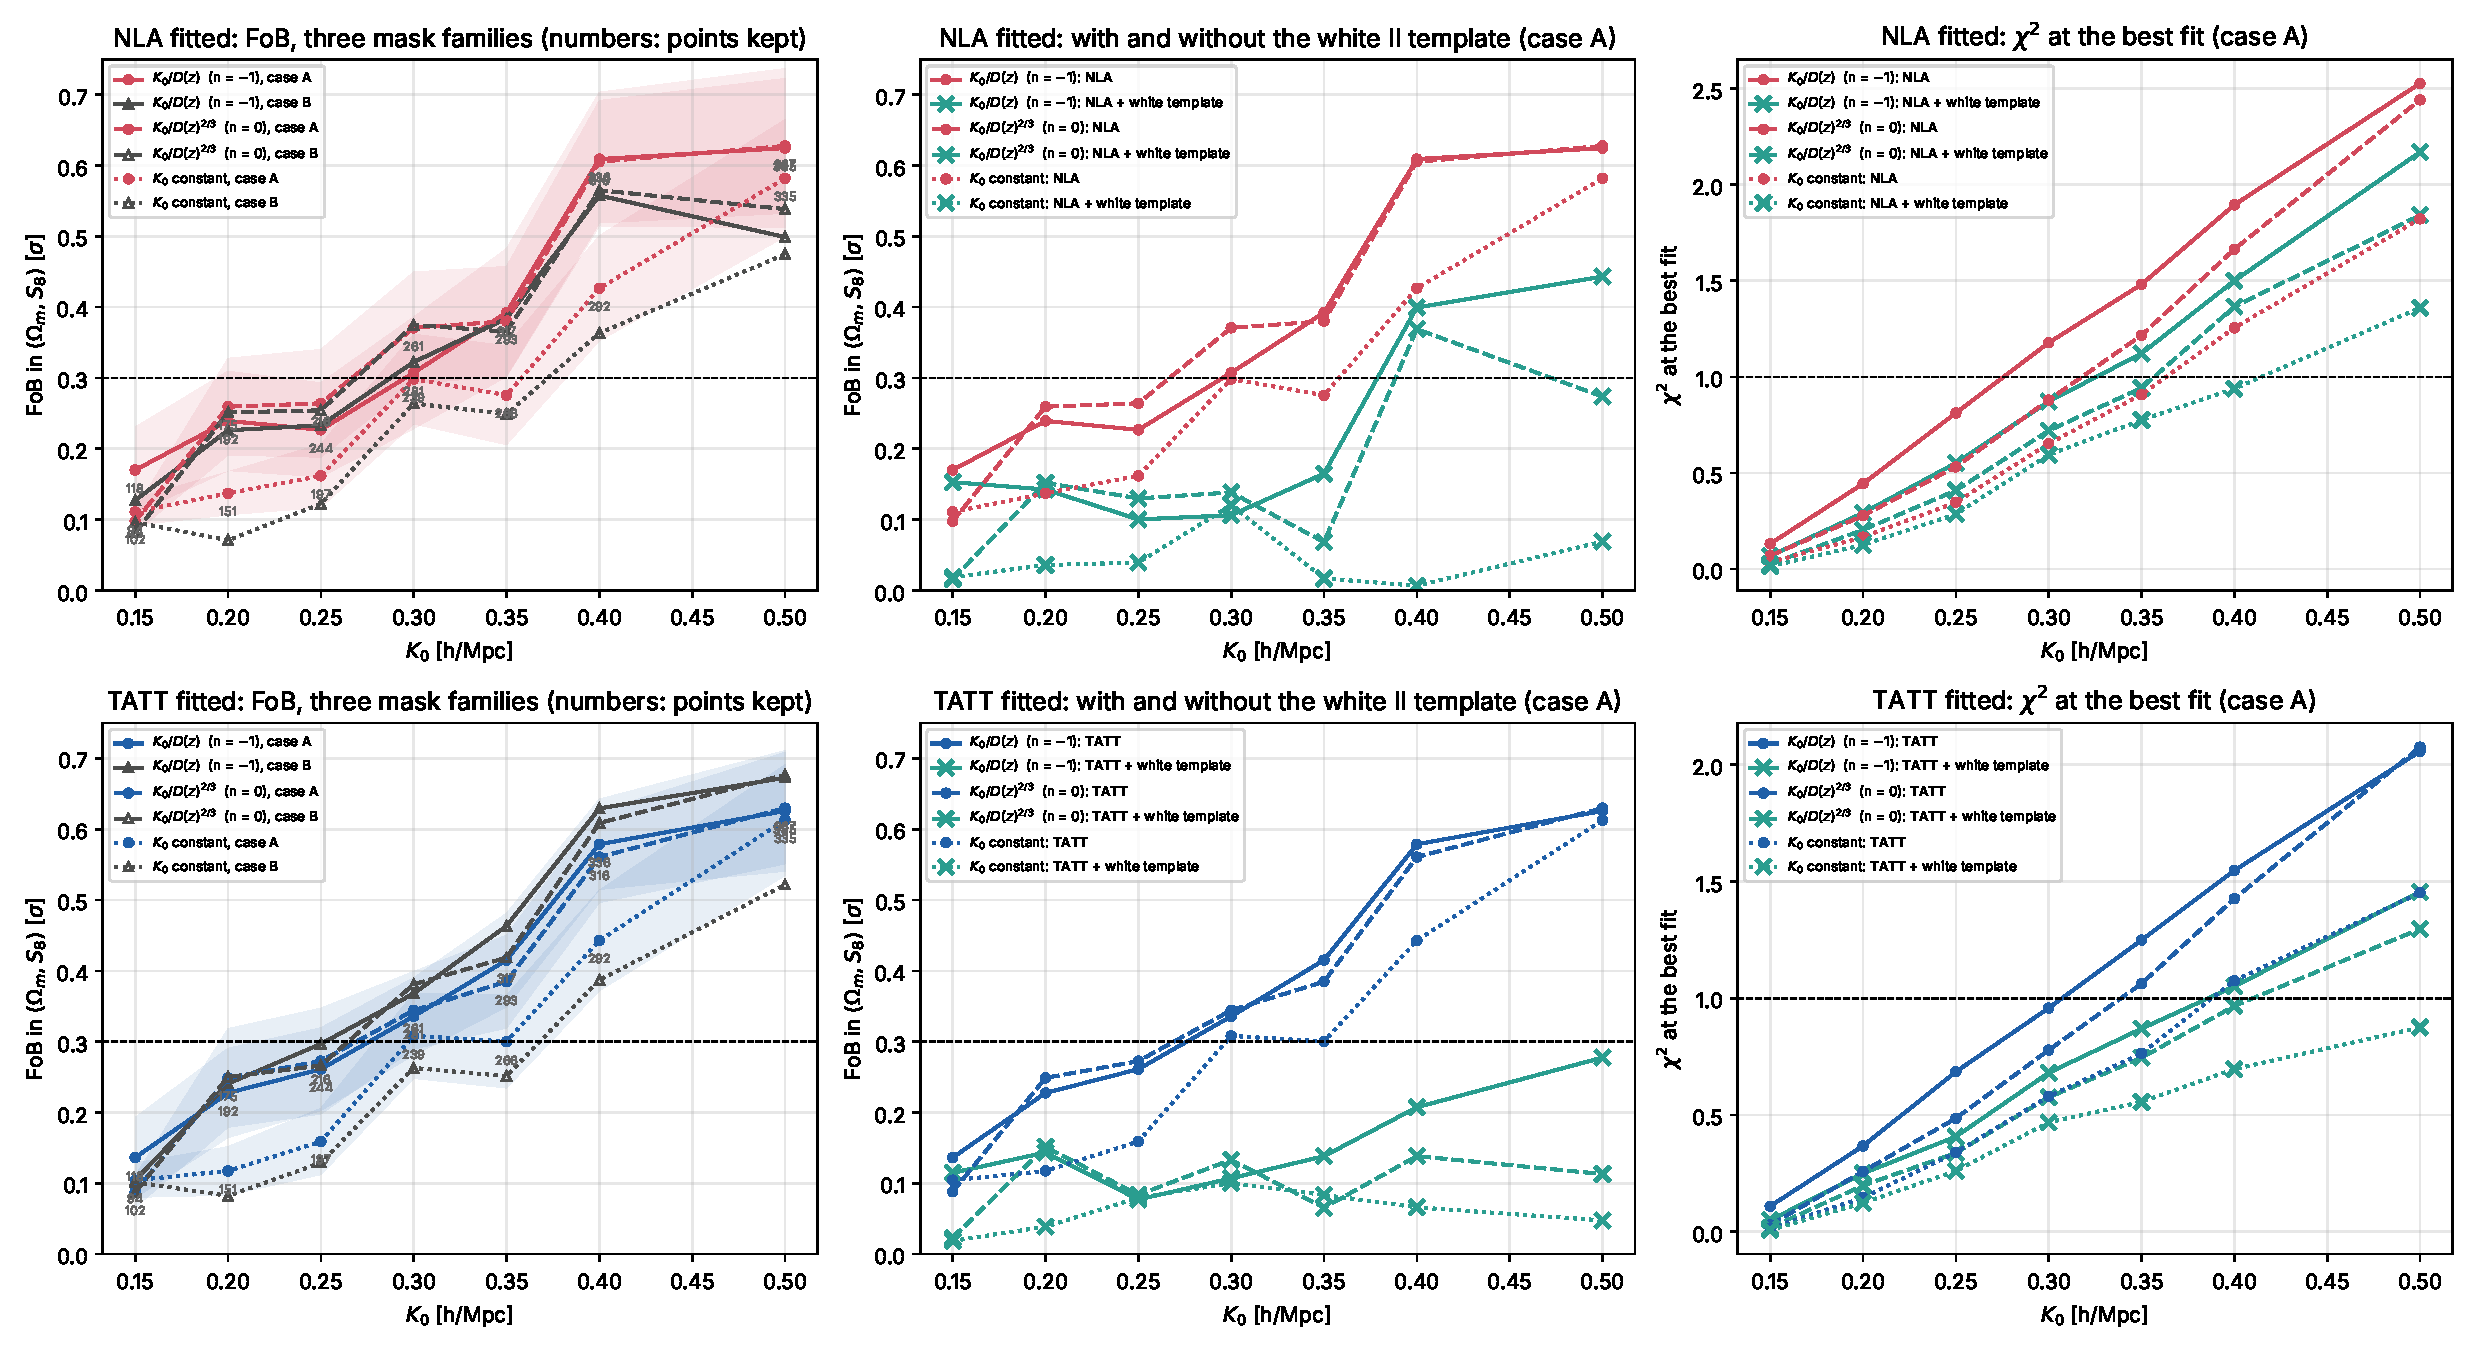
\includegraphics[width=\textwidth]{fig_mask_scan.pdf}
\caption{FoB (left: cases A and B; middle: with and without the white II template) and best-fit $\chi^2$ (right) against $K_0$ for the three families (solid $K_0/D$, dashed $K_0/D^{2/3}$, dotted constant), NLA fitted (top) and TATT fitted (bottom). Bands: FLAMINGO-noise uncertainty (case A). Numbers: data points kept of 1080.}\label{fig:scan}\end{figure}

\begin{table}[H]\centering\footnotesize\setlength{\tabcolsep}{3pt}
\caption{The mask scan. $\pm$: FoB uncertainty from the simulation's error bars.}\label{tab:scan}
\resizebox{\textwidth}{!}{%
\begin{tabular}{lcccrcccccc}
\toprule
family & $K_0$ & $k_{\rm UV}(z{=}0.5)$ & $k_{\rm UV}(z{=}2)$ & pts & FoB A: NLA / TATT & FoB B: NLA / TATT & $\chi^2$ NLA / TATT & + white template: NLA / TATT & $\delta S_8/\sigma$ NLA; TATT \\
\midrule
$K_0/D$ & 0.15 & 0.19 & 0.36 & 118 & 0.17 $\pm$ 0.06 / 0.14 $\pm$ 0.06 & 0.13 / 0.10 & 0.13 / 0.11 & 0.15 / 0.12 & +0.13; +0.09 \\
$K_0/D$ & 0.2 & 0.26 & 0.48 & 192 & 0.24 $\pm$ 0.07 / 0.23 $\pm$ 0.06 & 0.23 / 0.24 & 0.44 / 0.37 & 0.14 / 0.14 & +0.22; +0.19 \\
$K_0/D$ & 0.25 & 0.32 & 0.60 & 244 & 0.23 $\pm$ 0.07 / 0.26 $\pm$ 0.06 & 0.23 / 0.30 & 0.81 / 0.68 & 0.10 / 0.08 & +0.22; +0.24 \\
$K_0/D$ & 0.3 & 0.39 & 0.71 & 281 & 0.31 $\pm$ 0.08 / 0.34 $\pm$ 0.06 & 0.32 / 0.37 & 1.18 / 0.96 & 0.11 / 0.11 & +0.31; +0.31 \\
$K_0/D$ & 0.35 & 0.45 & 0.83 & 317 & 0.39 $\pm$ 0.09 / 0.41 $\pm$ 0.07 & 0.38 / 0.46 & 1.48 / 1.25 & 0.17 / 0.14 & +0.39; +0.41 \\
$K_0/D$ & 0.4 & 0.52 & 0.95 & 336 & 0.61 $\pm$ 0.09 / 0.58 $\pm$ 0.06 & 0.56 / 0.63 & 1.90 / 1.55 & 0.40 / 0.21 & +0.61; +0.57 \\
$K_0/D$ & 0.5 & 0.65 & 1.19 & 385 & 0.62 $\pm$ 0.11 / 0.63 $\pm$ 0.09 & 0.50 / 0.67 & 2.53 / 2.06 & 0.44 / 0.28 & +0.60; +0.63 \\
\midrule
$K_0/D^{2/3}$ & 0.15 & 0.18 & 0.27 & 102 & 0.10 $\pm$ 0.02 / 0.09 $\pm$ 0.02 & 0.08 / 0.09 & 0.07 / 0.03 & 0.02 / 0.02 & +0.09; +0.09 \\
$K_0/D^{2/3}$ & 0.2 & 0.24 & 0.36 & 175 & 0.26 $\pm$ 0.07 / 0.25 $\pm$ 0.07 & 0.25 / 0.25 & 0.28 / 0.26 & 0.15 / 0.15 & +0.25; +0.24 \\
$K_0/D^{2/3}$ & 0.25 & 0.30 & 0.45 & 216 & 0.26 $\pm$ 0.08 / 0.27 $\pm$ 0.07 & 0.25 / 0.27 & 0.53 / 0.49 & 0.13 / 0.08 & +0.26; +0.27 \\
$K_0/D^{2/3}$ & 0.3 & 0.36 & 0.54 & 261 & 0.37 $\pm$ 0.08 / 0.34 $\pm$ 0.06 & 0.38 / 0.38 & 0.88 / 0.78 & 0.14 / 0.13 & +0.37; +0.33 \\
$K_0/D^{2/3}$ & 0.35 & 0.42 & 0.62 & 293 & 0.38 $\pm$ 0.08 / 0.39 $\pm$ 0.07 & 0.36 / 0.42 & 1.22 / 1.06 & 0.07 / 0.07 & +0.37; +0.38 \\
$K_0/D^{2/3}$ & 0.4 & 0.48 & 0.71 & 316 & 0.60 $\pm$ 0.09 / 0.56 $\pm$ 0.06 & 0.56 / 0.61 & 1.66 / 1.43 & 0.37 / 0.14 & +0.60; +0.56 \\
$K_0/D^{2/3}$ & 0.5 & 0.59 & 0.89 & 367 & 0.63 $\pm$ 0.10 / 0.63 $\pm$ 0.08 & 0.54 / 0.68 & 2.44 / 2.08 & 0.27 / 0.11 & +0.59; +0.63 \\
\midrule
constant & 0.15 & 0.15 & 0.15 & 94 & 0.11 $\pm$ 0.02 / 0.10 $\pm$ 0.02 & 0.10 / 0.10 & 0.03 / 0.02 & 0.02 / 0.02 & +0.11; +0.10 \\
constant & 0.2 & 0.20 & 0.20 & 151 & 0.14 $\pm$ 0.03 / 0.12 $\pm$ 0.03 & 0.07 / 0.08 & 0.17 / 0.15 & 0.04 / 0.04 & +0.10; +0.10 \\
constant & 0.25 & 0.25 & 0.25 & 197 & 0.16 $\pm$ 0.04 / 0.16 $\pm$ 0.05 & 0.12 / 0.13 & 0.35 / 0.34 & 0.04 / 0.08 & +0.14; +0.14 \\
constant & 0.3 & 0.30 & 0.30 & 239 & 0.30 $\pm$ 0.06 / 0.31 $\pm$ 0.06 & 0.26 / 0.26 & 0.65 / 0.58 & 0.12 / 0.10 & +0.30; +0.30 \\
constant & 0.35 & 0.35 & 0.35 & 266 & 0.28 $\pm$ 0.07 / 0.30 $\pm$ 0.07 & 0.25 / 0.25 & 0.91 / 0.76 & 0.02 / 0.08 & +0.28; +0.30 \\
constant & 0.4 & 0.40 & 0.40 & 292 & 0.43 $\pm$ 0.07 / 0.44 $\pm$ 0.07 & 0.36 / 0.39 & 1.26 / 1.07 & 0.01 / 0.07 & +0.41; +0.44 \\
constant & 0.5 & 0.50 & 0.50 & 335 & 0.58 $\pm$ 0.08 / 0.61 $\pm$ 0.08 & 0.47 / 0.52 & 1.82 / 1.45 & 0.07 / 0.05 & +0.56; +0.60 \\
\bottomrule
\end{tabular}}
\end{table}

\paragraph{Reading.}
\begin{itemize}
\item \textbf{The 0.3$\sigma$ crossing sits at $K_0 \simeq 0.3$ in every family.} $K_0/D$: 0.31 / 0.34 at $K_0 = 0.3$ (281 points); $K_0/D^{2/3}$: 0.26 / 0.27 at 0.25 and 0.37 / 0.34 at 0.3 (crossing near 0.27, about 230 points); constant: 0.30 / 0.31 at 0.3 (239 points). Case B is within $+0.07$ of case A everywhere.
\item \textbf{At matched data volume the $1/D$ family is the most efficient.} 244 points with $K_0/D$ ($K_0 = 0.25$) give FoB 0.23 / 0.26; 239 points with a constant cut ($k = 0.3$) give 0.30 / 0.31; 261 points with $D^{-2/3}$ ($K_0 = 0.3$) give 0.37 / 0.34. The reason is not where the models fail in $k$ (the simulation says that is flat in $z$) but where the Roman bias comes from: the white II term and the small-$\theta$ $\xi_-$ of the low-redshift bins, which the $1/D$ family cuts hardest at low $z$. The redshift shape of the mask should therefore be chosen on the Roman side, and the $1/D$ family is a reasonable choice for the cosmic-shear mask even though it is not the shape of the simulation cuts.
\item \textbf{With the white template every family opens up.} $K_0/D$: 0.11 / 0.11 at $K_0 = 0.3$, 0.17 / 0.14 at 0.35, then NLA fails at 0.4 (0.40) while TATT stays at 0.21 to 0.28 to $K_0 = 0.5$. Constant cut: both models stay below 0.12 up to $k = 0.5\hmpc$ (NLA 0.007 to 0.12, TATT 0.02 to 0.10), with $\chi^2$ 0.9 to 1.4. $D^{-2/3}$: TATT below 0.14 everywhere, NLA 0.37 at 0.4. One nuisance parameter for the one-halo II term therefore moves the usable range from $k \simeq 0.3$ to at least $0.5\hmpc$ with a constant cut, and this is the configuration in which TATT is consistently the better model.
\item \textbf{Flat $z$-dependent cuts of Sec.~\ref{sec:roman} in this picture.} The TATT-shaped flat cut (0.22 to 0.29, 145 points) sits between the constant 0.2 and 0.25 rows (FoB 0.14 to 0.16); the constant 0.25 row (197 points, FoB 0.16 / 0.16, $\chi^2$ 0.35) is the simplest mask that keeps the TATT simulation cut's data volume with margin.
\end{itemize}

\section{GGL and 3x2pt with the FLAMINGO GI injected}\label{sec:3x2}
\paragraph{Set-up.} The 3x2pt data vector of \texttt{cocoa\_roman\_real} (2115 entries: 540 $\xi_+$, 540 $\xi_-$, 915 $\gamma_t$ for the 61 lens-source pairs after the standard exclusions, 120 $w(\theta)$; 15 $\theta$ bins, 2.5--250$'$) is computed with cosmolike (\texttt{cocoa/driver3x2.py}). Lenses and sources share \texttt{example1.nz}, as the dataset does; linear galaxy bias $b_i$ = (1.24, 1.36, 1.55, 1.71, 1.90, 2.15, 2.52, 2.44) (the wrappers' \texttt{B1\_FID}), no magnification, no point mass; Limber for $\gamma_t$ (required by the sim\_IA path) and for $w$, for truth and models alike. The truth is
\begin{equation}
d = \big[\text{GG + galaxy terms}\big](\theta_{\rm fid}, b_i) + \xi^{\rm IA}_{\rm FLAMINGO},
\end{equation}
with the FLAMINGO tables injected through sim\_IA: GI + II in $\xi_\pm$ (identical to the $\xi_{\rm FL}$ of Sec.~\ref{sec:roman}, checked to machine precision) and GI $= b_i\,n_i\,n_j\,P_{\delta E}$ in $\gamma_t^{ij}$; $w$ carries no IA. The model is native cosmolike NLA / TATT 3x2pt with $\Omega_m$, $A_s$, the eight $b_i$ ($[0.8, 3]$) and the IA parameters free (Sec.~\ref{sec:romantest} fit; $b_i$ enter through the same linear response as the cosmology, refreshed at the IA solution). The covariance is the Gaussian 3x2pt covariance (\texttt{cocoa/cov3x2.py}: flat-sky, $J_0/J_2/J_4$ bin averages, $N_E = \sigma_e^2/n_s$, $N_g = 1/n_l$ with $n_l = n_s$ = 41.3/8 per bin, 2415 deg$^2$, the IA spectra of the truth included in the signal part; its $\xi_\pm$ block reproduces the covariance of Sec.~\ref{sec:roman} exactly). Masks: IR/UV ($\alpha = 0.05$, GG + NLA baseline, monotonic rows) with a separate $K_0/D(z)$ per probe, $K_0^{\rm cs} \in \{0.2, 0.3\}$, $K_0^{\rm ggl} \in \{0.1, 0.15, 0.2, 0.3, 0.4\}$, $K_0^{\rm gc} = 0.2$. Two GGL configurations: all 61 pairs, and ``sources behind lenses'' ($s > l$, 28 pairs), the conservative choice. No FLAMINGO-noise band here (the $\xi$ Jacobian of Sec.~\ref{sec:translate} does not cover $\gamma_t$).

\paragraph{A property of this set-up.} With a shared lens/source $n(z)$ the same-bin $\gamma_t^{ii}$ is GI-dominated: at the FLAMINGO amplitude the GI term is $-1.7$ to $-4$ times the lensing signal in $\gamma_t^{ii}$ at $z$ = 0.2 to 1.5 (lensing by galaxies at the same redshift is weak, the alignment of their neighbours is not). Those pairs are therefore a direct measurement of $P_{\delta E}(k, z)$, with no II and no white term, and they decide the all-pairs results below.

\begin{figure}[H]\centering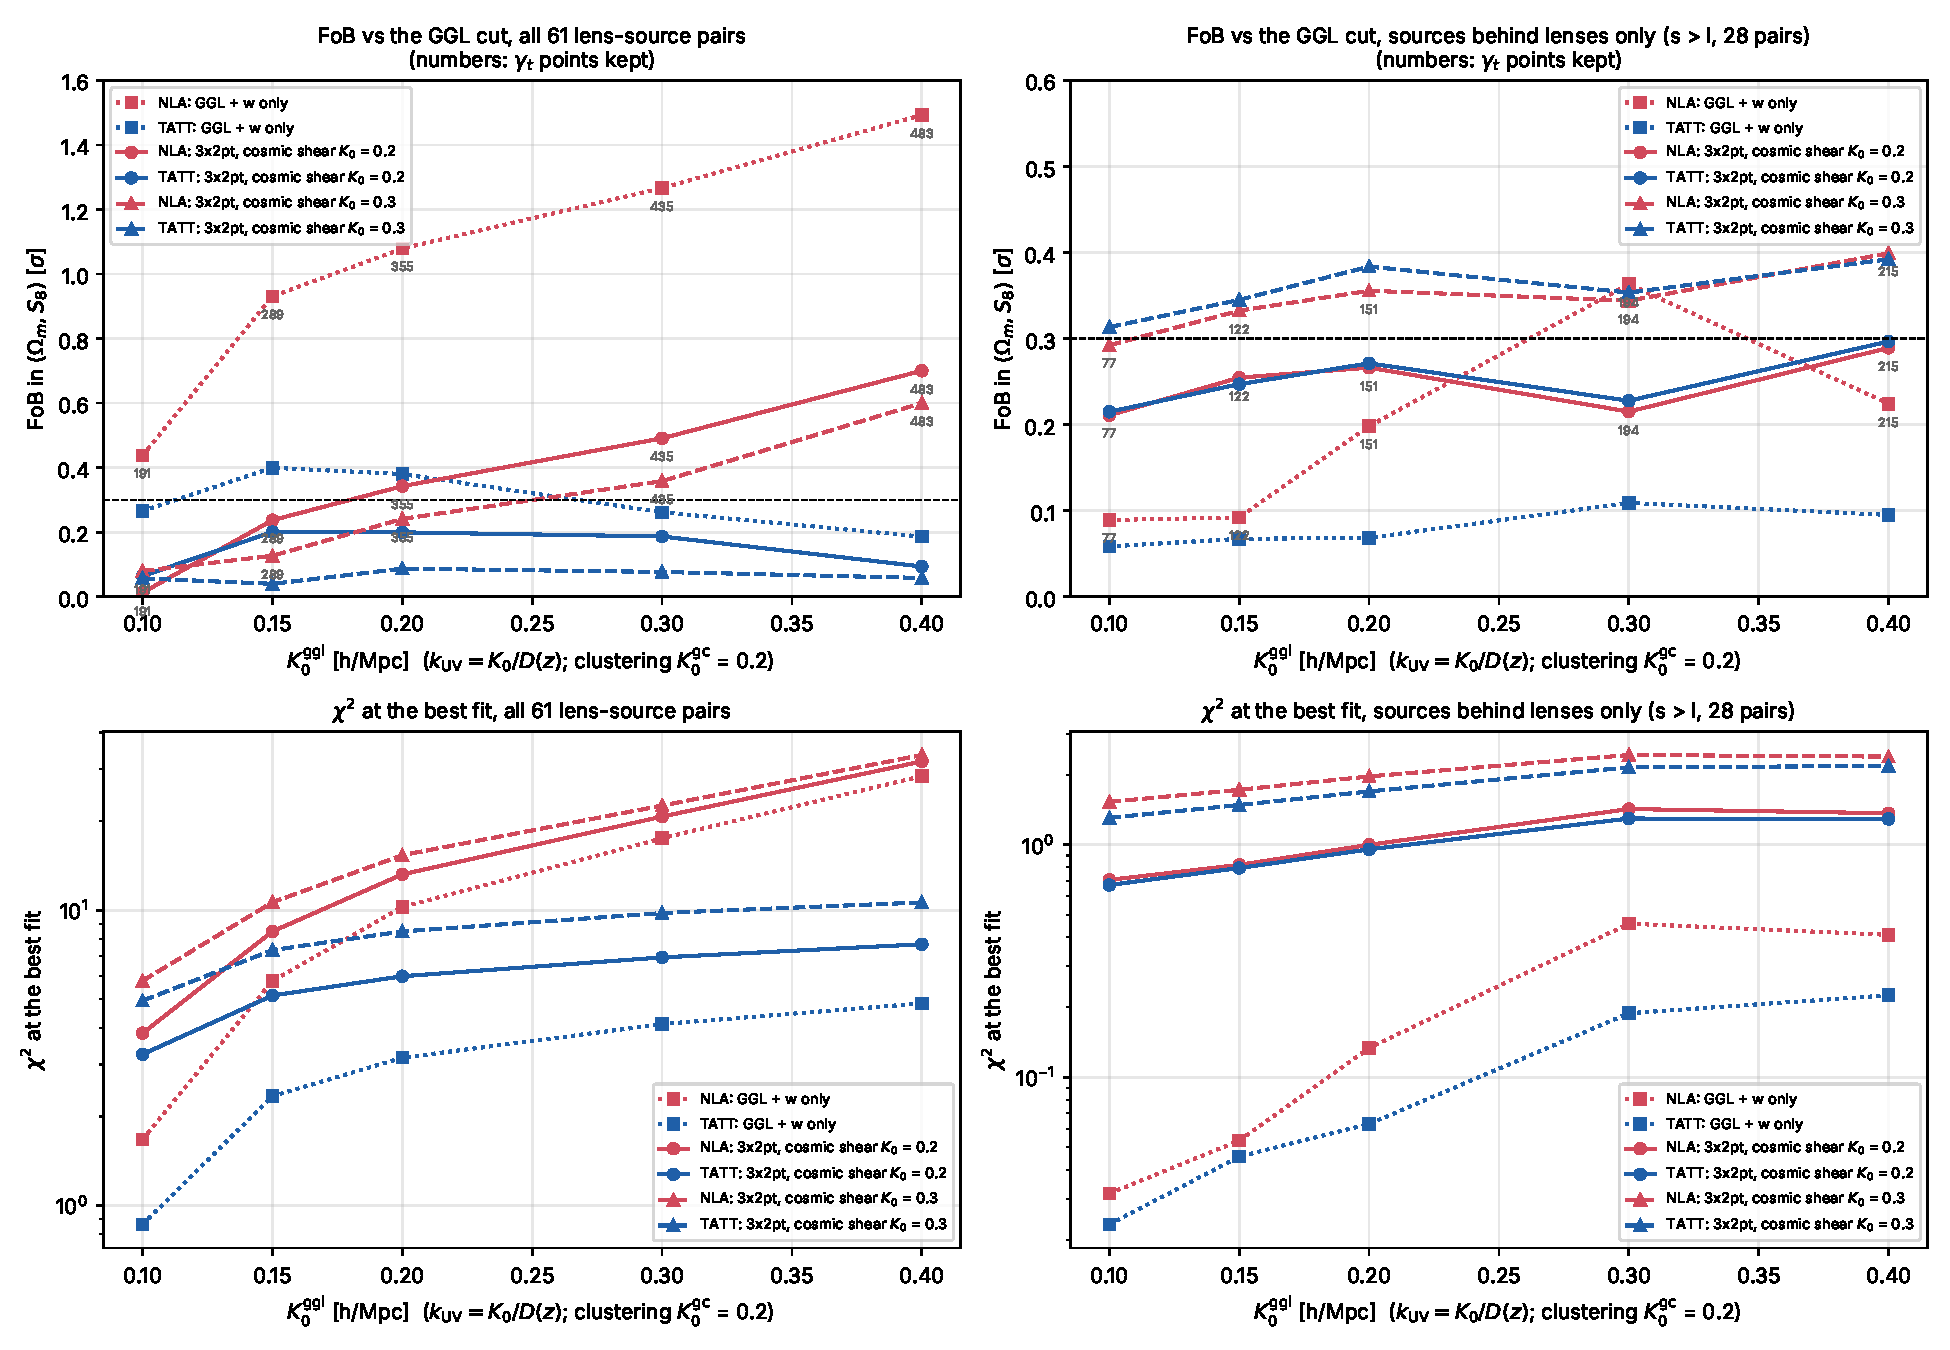
\includegraphics[width=\textwidth]{fig_ggl3x2.pdf}
\caption{Figure of bias (top) and best-fit $\chi^2$ (bottom) against the GGL cut $K_0^{\rm ggl}$ for GGL + $w$ alone (dotted) and 3x2pt with the cosmic-shear cut $K_0^{\rm cs}$ = 0.2 (solid) and 0.3 (dashed); NLA red, TATT blue. Left: all 61 lens-source pairs; right: sources behind lenses only. Numbers: $\gamma_t$ points kept.}\label{fig:3x2}\end{figure}

\begin{table}[H]\centering\footnotesize\setlength{\tabcolsep}{4pt}
\caption{GGL and 3x2pt results, all lens-source pairs. $K_0^{\rm gc} = 0.2$ throughout; $\xi_\pm$ points 192 ($K_0^{\rm cs}$ = 0.2) and 281 (0.3), $w$ points 48.}
\label{tab:3x2all}
\resizebox{\textwidth}{!}{%
\begin{tabular}{llcrccc}
\toprule
probes & $K_0^{\rm cs}$ & $K_0^{\rm ggl}$ & $\gamma_t$ pts & FoB NLA / TATT & $\chi^2$ NLA / TATT & $(\delta\Omega_m, \delta S_8)/\sigma$ NLA; TATT \\
\midrule
3x2pt & 0.2 & 0.1 & 191 & 0.01 / 0.06 & 3.8 / 3.2 & (+0.01, +0.00); (-0.03, -0.06) \\
3x2pt & 0.2 & 0.15 & 289 & 0.24 / 0.20 & 8.5 / 5.1 & (+0.14, -0.14); (-0.02, -0.20) \\
3x2pt & 0.2 & 0.2 & 355 & 0.34 / 0.20 & 13.2 / 6.0 & (+0.22, -0.17); (-0.10, -0.20) \\
3x2pt & 0.2 & 0.3 & 435 & 0.49 / 0.19 & 20.8 / 6.9 & (+0.35, -0.23); (-0.07, -0.19) \\
3x2pt & 0.2 & 0.4 & 483 & 0.70 / 0.09 & 31.9 / 7.7 & (+0.62, -0.16); (-0.06, -0.08) \\
3x2pt & 0.3 & 0.1 & 191 & 0.08 / 0.06 & 5.8 / 4.9 & (+0.06, +0.06); (+0.02, +0.06) \\
3x2pt & 0.3 & 0.15 & 289 & 0.13 / 0.04 & 10.6 / 7.3 & (+0.11, -0.03); (-0.03, -0.03) \\
3x2pt & 0.3 & 0.2 & 355 & 0.24 / 0.09 & 15.4 / 8.5 & (+0.21, -0.06); (-0.08, -0.04) \\
3x2pt & 0.3 & 0.3 & 435 & 0.36 / 0.08 & 22.6 / 9.8 & (+0.30, -0.11); (-0.07, -0.04) \\
3x2pt & 0.3 & 0.4 & 483 & 0.60 / 0.06 & 33.5 / 10.6 & (+0.55, -0.10); (-0.05, -0.04) \\
GGL+w & -- & 0.1 & 191 & 0.44 / 0.27 & 1.7 / 0.9 & (+0.17, -0.35); (+0.06, -0.24) \\
GGL+w & -- & 0.15 & 289 & 0.93 / 0.40 & 5.8 / 2.4 & (+0.28, -0.80); (-0.00, -0.39) \\
GGL+w & -- & 0.2 & 355 & 1.08 / 0.38 & 10.2 / 3.2 & (+0.46, -0.88); (-0.03, -0.38) \\
GGL+w & -- & 0.3 & 435 & 1.27 / 0.26 & 17.5 / 4.1 & (+0.73, -1.02); (-0.02, -0.26) \\
GGL+w & -- & 0.4 & 483 & 1.49 / 0.19 & 28.5 / 4.8 & (+0.99, -1.12); (-0.09, -0.15) \\
\bottomrule
\end{tabular}}
\end{table}
\begin{table}[H]\centering\footnotesize\setlength{\tabcolsep}{4pt}
\caption{As Table~\ref{tab:3x2all}, sources behind lenses only ($s > l$).}
\label{tab:3x2behind}
\resizebox{\textwidth}{!}{%
\begin{tabular}{llcrccc}
\toprule
probes & $K_0^{\rm cs}$ & $K_0^{\rm ggl}$ & $\gamma_t$ pts & FoB NLA / TATT & $\chi^2$ NLA / TATT & $(\delta\Omega_m, \delta S_8)/\sigma$ NLA; TATT \\
\midrule
3x2pt & 0.2 & 0.1 & 77 & 0.21 / 0.21 & 0.7 / 0.7 & (-0.01, +0.20); (-0.03, +0.20) \\
3x2pt & 0.2 & 0.15 & 122 & 0.26 / 0.25 & 0.8 / 0.8 & (-0.03, +0.24); (-0.04, +0.22) \\
3x2pt & 0.2 & 0.2 & 151 & 0.27 / 0.27 & 1.0 / 1.0 & (-0.07, +0.22); (-0.09, +0.22) \\
3x2pt & 0.2 & 0.3 & 194 & 0.21 / 0.23 & 1.4 / 1.3 & (-0.18, +0.08); (-0.18, +0.10) \\
3x2pt & 0.2 & 0.4 & 215 & 0.29 / 0.30 & 1.4 / 1.3 & (-0.15, +0.20); (-0.17, +0.20) \\
3x2pt & 0.3 & 0.1 & 77 & 0.29 / 0.31 & 1.5 / 1.3 & (-0.00, +0.29); (-0.01, +0.31) \\
3x2pt & 0.3 & 0.15 & 122 & 0.33 / 0.34 & 1.7 / 1.5 & (-0.06, +0.31); (-0.06, +0.32) \\
3x2pt & 0.3 & 0.2 & 151 & 0.36 / 0.38 & 2.0 / 1.7 & (-0.12, +0.30); (-0.12, +0.33) \\
3x2pt & 0.3 & 0.3 & 194 & 0.34 / 0.35 & 2.4 / 2.1 & (-0.24, +0.19); (-0.24, +0.20) \\
3x2pt & 0.3 & 0.4 & 215 & 0.40 / 0.39 & 2.4 / 2.2 & (-0.23, +0.26); (-0.24, +0.26) \\
GGL+w & -- & 0.1 & 77 & 0.09 / 0.06 & 0.0 / 0.0 & (+0.01, -0.09); (+0.01, -0.06) \\
GGL+w & -- & 0.15 & 122 & 0.09 / 0.07 & 0.1 / 0.1 & (+0.02, -0.09); (+0.01, -0.07) \\
GGL+w & -- & 0.2 & 151 & 0.20 / 0.07 & 0.1 / 0.1 & (+0.02, -0.20); (+0.02, -0.07) \\
GGL+w & -- & 0.3 & 194 & 0.36 / 0.11 & 0.5 / 0.2 & (+0.05, -0.36); (+0.02, -0.11) \\
GGL+w & -- & 0.4 & 215 & 0.22 / 0.10 & 0.4 / 0.2 & (+0.07, -0.22); (+0.03, -0.09) \\
\bottomrule
\end{tabular}}
\end{table}

\paragraph{Reading.}
\begin{itemize}
\item \textbf{With all pairs, GGL separates the two models at the cosmology level.} 3x2pt with $K_0^{\rm cs} = 0.2$: NLA crosses $0.3\sigma$ at $K_0^{\rm ggl} \simeq 0.18$ (0.24 at 0.15, 0.34 at 0.2, 0.49 at 0.3, 0.70 at 0.4) while TATT stays at 0.06 to 0.20 up to 0.4; with $K_0^{\rm cs} = 0.3$ NLA reaches 0.3 at $K_0^{\rm ggl} \simeq 0.25$ and TATT stays below 0.09. The NLA shift is in $\Omega_m$ ($+0.2$ to $+0.6\sigma$) with $S_8$ going the other way. GGL + $w$ alone is worse still for NLA (FoB 0.4 at $K_0^{\rm ggl} = 0.1$, 1.1 at 0.2; $\delta S_8 = -0.35$ to $-1.1\sigma$ of the much larger lens-only error), and TATT improves on it by a factor 2 to 8 but is not clean either (0.19 to 0.40). The reason is the same-bin $\gamma_t$: NLA with a power-law $A_1(z)$ cannot follow the measured $P_{\delta E}$ (the dip to 0.8 of $C_1 P_{\rm NL}$ at $0.3 < k < 1$ and the amplitude evolution), TATT can, but only in an odd corner of its parameter space: every all-pairs TATT fit lands at $A_2 \simeq 0.05$ with $\eta_2 = +5$, the edge of the prior, i.e.\ $A_2(z) \simeq 0.04$ at $z = 0.5$ rising to 1.3 at $z = 2$, with $b_{\rm TA} \le 0.14$, far from the $A_2 \simeq -1$ that the II-driven cosmic-shear fit selects. The fit is using the tidal-torquing term only in the highest-redshift lens bins, where the $z = 2$ snapshot has the anomalous $A_2 > 0$ of Sec.~\ref{sec:gof}; it is a boundary solution, not a physical TATT description of $P_{\delta E}$. A first pass with fewer starting points found higher-$\chi^2$ local minima on a second branch ($A_2 \simeq 0.6$, $\eta_2 \simeq -4.5$, $b_{\rm TA} \simeq 0.3$) with FoB 0.02 to 0.14; the numbers quoted here are from the denser start grid (both branches seeded), which lowered $\chi^2$ by up to a factor 2 and moved the TATT FoB by up to $\pm0.1$.
\item \textbf{The 3x2pt TATT fit is nearly unbiased even where cosmic shear alone is not.} At $K_0^{\rm cs} = 0.3$ cosmic shear alone gives TATT FoB 0.34 ($+0.3\sigma$ in $S_8$, Sec.~\ref{sec:romantest}); in 3x2pt with all pairs it is 0.04 to 0.09. The GGL GI term pins the IA amplitudes, which removes the degeneracy direction through which the white II excess moved $S_8$ in cosmic shear; the excess then stays in the residual ($\chi^2$ 3 to 11 for 600 to 800 points, still well below one per point). Given the boundary solution above, this should be read as ``the TATT parameter space is large enough to absorb the same-bin GI over the fitted range'' rather than as a validation of TATT.
\item \textbf{With sources behind lenses only, 3x2pt behaves like cosmic shear.} The GI term in $\gamma_t^{l s}$ with $s > l$ is small, the lens probes mainly add constraining power, and both models return to the common $S_8$ shift of Sec.~\ref{sec:romantest}: FoB 0.21 to 0.29 ($K_0^{\rm cs} = 0.2$) and 0.29 to 0.40 ($K_0^{\rm cs} = 0.3$) for NLA and TATT alike, almost independent of $K_0^{\rm ggl}$. GGL + $w$ alone is then clean for both models up to $K_0^{\rm ggl} = 0.2$ (FoB $\le 0.2$) and NLA fails at 0.3 (0.36).
\item \textbf{Cuts for the lens probes.} In the conservative (behind-only) configuration the GGL cut is not what limits the 3x2pt bias; the cosmic-shear cut is, and the plan's $K_0^{\rm ggl} = 0.2$ is safe for both models ($K_0^{\rm ggl} \le 0.2$ from the GGL-only test for NLA, no limit found for TATT up to 0.4). If the same-bin pairs are kept, the GGL cut must be set per model: $K_0^{\rm ggl} \lesssim 0.15$ for NLA at $K_0^{\rm cs} = 0.2$, no limit found for TATT up to 0.4; TATT then does reduce the cosmological bias, but through a prior-boundary solution driven by the $z \ge 1.5$ snapshots, so this configuration needs the TATT priors and the high-$z$ snapshots settled before it can be used.
\item \textbf{Caveats.} Gaussian covariance; $n_l = n_s$ and a shared $n(z)$ (the real lens sample will differ); linear bias and no magnification; Limber $\gamma_t$ and $w$; all all-pairs TATT fits sit at the $\eta_2 = +5$ bound and several at $b_{\rm TA} = 0$ (listed in \texttt{ggl3x2.csv}); the first-pass results are kept as \texttt{ggl3x2\_*\_v1.json}; the IR/UV mask for $\gamma_t$ uses the GG + NLA baseline. The same-bin GI dominance is a statement about this set-up, and the Roman lens selection decides how much of it survives.
\end{itemize}

\section{Scale-cut proposals and reading}
\begin{enumerate}
\item \textbf{Simulation-only, significance based (GoF, $N_s$ fixed).} $k_{\max}(z)\simeq0.1\hmpc$ for NLA and $0.25$--$0.3\hmpc$ for TATT, flat in $z$ over the core. Conservative by construction (FLAMINGO's errors are 2--5\% at these $k$). In Roman the NLA cut keeps 9 points; the TATT cut keeps 145 with FoB $0.22\pm0.09$ for both models.
\item \textbf{Simulation-only, accuracy based (anchored, 5\%/10\%).} GI alone: both models accurate to 5\% up to $k\simeq0.16$--$0.3$. GI+II at 10\%: NLA $0.1$, TATT $0.22$--$0.39$. The II accuracy is limited by the white term, not by the perturbative modelling.
\item \textbf{Roman-based (FoB $<0.3$).} Both models: $k_{\rm UV}(z=1)\lesssim0.37\hmpc$ (flat cut) or $K_0\lesssim0.3$ ($K_0/D$ family), set by the white II term; with that term modelled, $\lesssim0.4$--$0.6$ with TATT preferred beyond 0.4.
\item \textbf{Mask shape (Sec.~\ref{sec:scan}).} The $0.3\sigma$ crossing is at $K_0\simeq0.3$ for all three redshift shapes; at matched data volume $K_0/D(z)$ is the most efficient for the Roman bias even though the simulation cuts are flat in $z$. With the white II template a constant cut passes to $k\simeq0.5\hmpc$ for both models.
\item \textbf{Lens probes (Sec.~\ref{sec:3x2}).} With sources behind lenses only, the plan's $K_0^{\rm ggl}=0.2$ is safe for both models and the 3x2pt bias is set by the cosmic-shear cut. If same-bin lens-source pairs are kept, GGL measures $P_{\delta E}$ directly: NLA then needs $K_0^{\rm ggl}\lesssim0.15$ while TATT stays at or below $0.2\sigma$ up to 0.4, but through a solution at the $\eta_2$ prior bound driven by the $z\ge1.5$ snapshots.
\item \textbf{Recommendation.} For the paper's TATT-on-FLAMINGO analysis a flat $k_{\rm UV}\simeq0.3\hmpc$ (or $K_0=0.15$--$0.2$ in the $/D(z)$ family, Sec.~\ref{sec:kuvz}) is defensible from the simulation alone and gives FoB $0.2$--$0.25$ in Roman for either model. Going beyond it requires a decision on the white one-halo II term: either declare it part of the truth (then no cut above $0.3$ passes $0.3\sigma$ and TATT does not help), or add it to the model (then $0.4$--$0.6$ is reachable and the NLA/TATT difference appears).
\end{enumerate}

\appendix
\section{Pipeline checks}\label{app:checks}
\begin{itemize}
\item cosmolike build: cocoa-cosmolike-core b811ae0 + \texttt{core-sim-IA.patch}; cocoa\_roman\_real 0559522 + \texttt{roman\_real-sim-IA.patch}; compiled with \texttt{-DSIM\_KMIN\_HMPC=1e-6 -DSIM\_KMAX\_HMPC=0} (default build trims tables to 0.5--7$\hmpc$, which gives $\dchi\sim1000$ on the 0.35/D mask).
\item \texttt{example1.modelvector} reproduced to $3\times10^{-5}$ median; $n(z)$ read with cocoa's left-edge convention.
\item Conversion: term-by-term identical to the analysis spectra; \texttt{sim\_IA.c}'s own conversion of the raw files gives the same $\xi_{\rm IA}$ to $2.5\times10^{-9}$; the injected $\xi_{\rm IA}$ over native NLA with the report's $a_{\rm NLA}(z)$ is 1.01--1.05 at $\theta\ge21'$.
\item NLA power law as tables versus native NLA: $\dchi=0.001$ on the masks; null fit on it: FoB 0.01. Fine $z$ grid ($\Delta z=0.025$) versus the 13 snapshots: 0.26--1.2 on the masks, FoB unchanged within noise.
\item Native TATT versus TATT tables differ by its B modes ($\dchi=41$ for the Part~1a fiducial), absent on the sim path; at the Roman best fits TATT's own B modes are worth 0.06--0.24.
\item Nesting: native TATT($A_2=b_{\rm TA}=0$) $=$ native NLA exactly. Linearised versus exact non-linear fits: identical.
\item Inputs re-checked against the \texttt{hinfo} files (7 November): $N_{\rm gal}$ identical, $e_{\rm rms}$ identical to three decimals, spectra byte-identical; no result changes.
\item Python Limber mishandles a white $P_{EE}$ (ringing from the $\ell$ taper); cosmolike gives the analytic $\theta^{-2}$ law.
\end{itemize}

\section{Code}
Base: \texttt{/tmp/claude-0/out/roman\_dchi2/}. Inputs: \texttt{tatt\_fit/fit\_tatt\_flamingo.py} (conversion, TATT model), FLAMINGO \texttt{psdata/PS}, \texttt{cocoa\_roman\_real/data}.
\begin{itemize}\small
\item \texttt{cocoa/cosmolike\_driver.py}: cosmolike interface (CAMB at D3A, native NLA/TATT, sim tables, $\xi_\pm$ vector). \texttt{cocoa/validate\_cosmolike.py}, \texttt{cocoa/verify\_injection.py}: checks.
\item \texttt{v2/flamingo\_truth.py}: fold-combined spectra, errors, $N_s$, smoothed truth. \texttt{v2/fit\_models.py}: v2 fits (free $N_s$) $\rightarrow$ \texttt{v2/fits.npz}.
\item \texttt{cocoa/cosmolike\_xi\_ia.py}: FLAMINGO and model tables, $\xi_{\rm IA}$, IR/UV masks $\rightarrow$ \texttt{run/cosmolike\_xi\_ia.npz}; \texttt{cocoa/analyze\_cosmolike.py}: $\dchi$ tables, Gaussian covariance.
\item \texttt{cocoa/translate\_matrix.py}: cell Jacobian $\mathsf{J}$, matrix $\mathsf{A}$; \texttt{cocoa/summary\_kmax.py}: GoF/$\dchi$/weight figures (\texttt{fig\_kmax\_*}).
\item \texttt{cocoa/bias\_analysis.py}: fit machinery; \texttt{cocoa/bias\_v2.py}: bounded priors, multi-start, B modes, raw, noise propagation, exact fits; \texttt{cocoa/bias\_diag.py}, \texttt{bias\_diag2.py}: injection null tests, per-bin NLA, GI/II split, large angles; \texttt{cocoa/bias\_white.py}, \texttt{white\_diag.py}, \texttt{bias\_phys.py}, \texttt{bias\_wtemplate.py}: white II excess decomposition, $\theta^{-2}$ check, extension test, white template; \texttt{cocoa/plot\_bias\_v2.py}, \texttt{plot\_white.py}, \texttt{plot\_final.py}: figures.
\item \texttt{v3/v3\_flamingo.py}: fixed-$N_s$ bounded fits, four criteria, cuts, amplitudes $\rightarrow$ \texttt{v3.npz}, \texttt{cuts.csv}, \texttt{combined.csv}, \texttt{amplitudes.csv}, \texttt{fig\_v3\_*}. \texttt{v3/v3\_roman.py}, \texttt{plot\_v3\_roman.py}: $z$-dependent masks, Roman $\dchi$ and FoB $\rightarrow$ \texttt{roman\_results.csv}, \texttt{masks\_v3.npz}.
\item \texttt{v3/roman\_test.py}, \texttt{plot\_roman\_test.py}: the Roman test with controls $\rightarrow$ \texttt{roman\_test.json/csv}, \texttt{fig\_roman\_test}. \texttt{v3/roman\_mcmc.py}: emcee check $\rightarrow$ \texttt{mcmc\_*.json}, \texttt{chain\_*.npy}.
\item \texttt{v3/plot\_kuv\_z.py}: Fig.~\ref{fig:kuvz}. \texttt{v3/knl\_scaling.py}: Sec.~\ref{sec:knl} ($k_{\rm NL}(z)$, $n_{\rm eff}$, power-law fits, profiles) $\rightarrow$ \texttt{knl.csv}, \texttt{knl.json}, \texttt{fig\_knl\_z}, \texttt{fig\_knl\_fit}.
\item \texttt{v3/mask\_scan.py}: Sec.~\ref{sec:scan} (three mask families, cases A/B, white template) $\rightarrow$ \texttt{mask\_scan.json/csv}, \texttt{masks\_scan.npz}. \texttt{v3/plot\_scan\_3x2.py}: \texttt{fig\_mask\_scan}, \texttt{fig\_ggl3x2}, \texttt{mask\_scan.csv}, \texttt{ggl3x2.csv}.
\item \texttt{cocoa/driver3x2.py}: cosmolike 3x2pt driver (lens sample, linear bias, Limber $\gamma_t$/$w$, sim\_IA in $\gamma_t$); \texttt{cocoa/cov3x2.py}: Gaussian 3x2pt covariance $\rightarrow$ \texttt{analysis/cov3x2\_gauss\_d3a.npy}; \texttt{v3/ggl3x2.py}: Sec.~\ref{sec:3x2} (parts \texttt{all}, \texttt{3x2\_behind}, \texttt{ggl\_behind}) $\rightarrow$ \texttt{ggl3x2\_*.json}, \texttt{dv3x2\_flam.npz}.
\item \texttt{report/summary.tex}: this document.
\end{itemize}
\end{document}
